\chapter{Resultados Computacionais} \label{chp:resultados}

Neste capítulo são descritos os  experimentos realizados para avaliar a eficácia
das  diversas  abordagens  propostas   nesta  dissertação.  Este  capítulo  está
organizado  da seguinte  maneira: a  Seção~\ref{sec:prep} contém  as informações
sobre os  pré-processamentos, seguida da Seção~\ref{sec:modelos},  que apresenta
os resultados dos modelos de \gls{pli} e \gls{plim} desenvolvidos.

%   dos   modelos   matemáticos   propostos  nas   Seções   \ref{sec:dmfm-pma}   e
% \ref{sec:ab-pma} juntamente  com o  impacto dos pré-processamentos  descritos na
% Seção  \ref{subsec:prep};   as  relaxações   lagrangianas  descritas   na  Seção
% \ref{sec:rl-pma}   e  as   variações  do   \gls{brkga}  apresentadas   na  Seção
% \ref{sec:brkga}.

As estratégias apresentadas foram implementadas  em C++, os programas compilados
com GCC  versão 7.5.0, usando o  nível de otimização -O3.  Os experimentos foram
realizados em um  processador Intel(R) Xeon(R) CPU E5-2630 v4  com 10 núcleos de
2.20  GHz  cada  e 64GB  de  memória  RAM.  A  execução ocorreu  em  um  sistema
operacional Linux Ubuntu 18.04 de 64  bits. Os experimentos foram realizados sob
um    conjunto    de   40    instâncias    geradas    e   disponibilizadas    em
\url{https://github.com/cvaraujo/QoS-MRP-Instances}.

\section{Pré-processamentos} \label{sec:prep}

Esta seção apresenta  os resultados relacionados às fixações de  variáveis com a
aplicação dos  pré-processamentos apresentados  na Seção~\ref{sec:prep-modelos}.
Para computar problemas de \gls{sp} e \gls{sprc} utilizaram-se as implementações
fornecidas pela biblioteca  Boost C++\footnote{\url{https://www.boost.org/}}. Os
resultados  encontram-se na  Tabela~\ref{tab:prep}. A  primeira coluna  contém a
identificação   da   instância,   as    três   colunas   seguintes   apresentam,
respectivamente,  o número  de nós  do grafo  ($|V|$), número  de nós  terminais
($|D|$) e quantidade de arcos ($|A|$).  A coluna ``MVE'' informa a quantidade de
nós que podem ser removidos da  instância pelo processamento em questão. A mesma
lógica se aplica às colunas ``MAE'' e ``SAE'', que indicam a quantidade de arcos
removidos e a quantidade  de variáveis $f_{ij}^{k} = 0$ para todo  $k \in D \cup
S$ e $(i, j) \in A$, respectivamente. A coluna ``Rem. SAE ($\%$)'' apresenta, em
porcentagens,  os valores  da coluna  ``SAE''. As  colunas ``Rem.  |V|'', ``Rem.
|A|'' e ``Rem.  |D|'' correspondem, respectivamente, aos nós,  arcos e terminais
removidos do grafo após aplicação  dos três pré-processamentos para a instância.
Por  fim,  a  coluna  ``Tempo''  apresenta   o  tempo,  em  segundos,  dos  três
procedimentos.
\newpage
% Tabela
\begin{table}[!ht]
\centering
\resizebox{\textwidth}{!}{%
\begin{tabular}{llrlrlrlrlrlrlrlrlrlrlr}
\hline
\multicolumn{1}{c}{Instância} &  & \multicolumn{1}{c}{\textbf{|V|}} &  & \multicolumn{1}{c}{\textbf{|D|}} &  & \multicolumn{1}{c}{\textbf{|A|}} &  & \multicolumn{1}{c}{\textbf{MVE}} &  & \multicolumn{1}{c}{\textbf{MAE}} &  & \multicolumn{1}{c}{\textbf{SAE}} &  & \multicolumn{1}{c}{\begin{tabular}[c]{@{}c@{}}\textbf{Rem.}\\ \textbf{SAE} (\%)\end{tabular}} &  & \multicolumn{1}{c}{\begin{tabular}[c]{@{}c@{}}\textbf{Rem.}\\ \textbf{|V|}\end{tabular}} &  & \multicolumn{1}{c}{\begin{tabular}[c]{@{}c@{}}\textbf{Rem.}\\ \textbf{|A|}\end{tabular}} &  & \multicolumn{1}{c}{\begin{tabular}[c]{@{}c@{}}\textbf{Rem.}\\ \textbf{|D|}\end{tabular}} &  & \multicolumn{1}{c}{\begin{tabular}[c]{@{}c@{}}\textbf{Tempo}\end{tabular}} \\ \hline
washington-50-10-6 &  & 10 &  & 6 &  & 46 &  & 1 &  & 11 &  & 156 &  & 33,9 &  & 3 &  & 20 &  & 0 &  & 0 \\
washington-50-20-11 &  & 20 &  & 11 &  & 184 &  & 0 &  & 33 &  & 1508 &  & 41,0 &  & 2 &  & 49 &  & 0 &  & 0 \\
washington-50-30-15 &  & 30 &  & 15 &  & 420 &  & 2 &  & 82 &  & 4925 &  & 39,1 &  & 5 &  & 128 &  & 0 &  & 0 \\
washington-50-40-23 &  & 40 &  & 23 &  & 830 &  & 1 &  & 184 &  & 17015 &  & 51,3 &  & 4 &  & 230 &  & 0 &  & 1 \\
washington-50-50-28 &  & 50 &  & 28 &  & 1248 &  & 6 &  & 321 &  & 31422 &  & 50,4 &  & 10 &  & 527 &  & 0 &  & 2 \\
washington-50-60-35 &  & 60 &  & 35 &  & 1812 &  & 9 &  & 412 &  & 56068 &  & 51,6 &  & 13 &  & 823 &  & 0 &  & 4 \\
washington-50-70-37 &  & 70 &  & 37 &  & 2516 &  & 2 &  & 707 &  & 86755 &  & 49,3 &  & 6 &  & 803 &  & 0 &  & 21 \\
washington-50-80-39 &  & 80 &  & 39 &  & 3592 &  & 12 &  & 1051 &  & 126159 &  & 43,9 &  & 15 &  & 1883 &  & 0 &  & 32 \\
washington-50-90-51 &  & 90 &  & 51 &  & 4218 &  & 14 &  & 1049 &  & 198888 &  & 52,4 &  & 19 &  & 1775 &  & 0 &  & 34 \\
washington-50-100-45 &  & 100 &  & 45 &  & 4416 &  & 31 &  & 1025 &  & 180369 &  & 40,8 &  & 33 &  & 2297 &  & 0 &  & 44 \\ \hline
washington-75-10-4 &  & 10 &  & 4 &  & 32 &  & 0 &  & 7 &  & 89 &  & 27,8 &  & 0 &  & 7 &  & 0 &  & 0 \\
washington-75-20-12 &  & 20 &  & 12 &  & 126 &  & 1 &  & 12 &  & 923 &  & 36,6 &  & 2 &  & 24 &  & 0 &  & 0 \\
washington-75-30-16 &  & 30 &  & 16 &  & 318 &  & 0 &  & 39 &  & 4190 &  & 43,9 &  & 1 &  & 44 &  & 0 &  & 0 \\
washington-75-40-21 &  & 40 &  & 21 &  & 538 &  & 2 &  & 40 &  & 9892 &  & 46,0 &  & 6 &  & 135 &  & 3 &  & 1 \\
washington-75-50-30 &  & 50 &  & 30 &  & 876 &  & 0 &  & 212 &  & 22354 &  & 51,0 &  & 4 &  & 259 &  & 0 &  & 3 \\
washington-75-60-25 &  & 60 &  & 25 &  & 1256 &  & 3 &  & 384 &  & 27572 &  & 36,6 &  & 11 &  & 539 &  & 0 &  & 3 \\
washington-75-70-42 &  & 70 &  & 42 &  & 1700 &  & 2 &  & 339 &  & 63943 &  & 53,7 &  & 5 &  & 470 &  & 0 &  & 17 \\
washington-75-80-48 &  & 80 &  & 48 &  & 2504 &  & 3 &  & 490 &  & 106488 &  & 53,2 &  & 11 &  & 825 &  & 0 &  & 30 \\
washington-75-90-47 &  & 90 &  & 47 &  & 3034 &  & 2 &  & 942 &  & 132330 &  & 48,5 &  & 8 &  & 1182 &  & 0 &  & 74 \\
washington-75-100-52 &  & 100 &  & 52 &  & 3792 &  & 4 &  & 1179 &  & 184042 &  & 48,5 &  & 6 &  & 1455 &  & 0 &  & 86 \\ \hline
washington-100-10-6 &  & 10 &  & 6 &  & 18 &  & 4 &  & 0 &  & 30 &  & 16,7 &  & 5 &  & 4 &  & 1 &  & 0 \\
washington-100-20-10 &  & 20 &  & 10 &  & 98 &  & 2 &  & 5 &  & 651 &  & 33,2 &  & 3 &  & 10 &  & 0 &  & 0 \\
washington-100-30-12 &  & 30 &  & 12 &  & 206 &  & 8 &  & 19 &  & 1466 &  & 23,7 &  & 9 &  & 46 &  & 1 &  & 0 \\
washington-100-40-18 &  & 40 &  & 21 &  & 422 &  & 1 &  & 29 &  & 5515 &  & 32,7 &  & 2 &  & 49 &  & 0 &  & 1 \\
washington-100-50-27 &  & 50 &  & 27 &  & 596 &  & 3 &  & 94 &  & 10405 &  & 34,9 &  & 8 &  & 154 &  & 1 &  & 2 \\
washington-100-60-34 &  & 60 &  & 34 &  & 854 &  & 2 &  & 99 &  & 26131 &  & 51,0 &  & 9 &  & 305 &  & 5 &  & 5 \\
washington-100-70-39 &  & 70 &  & 39 &  & 1204 &  & 3 &  & 276 &  & 37123 &  & 44,0 &  & 14 &  & 471 &  & 2 &  & 7 \\
washington-100-80-32 &  & 80 &  & 32 &  & 1764 &  & 3 &  & 442 &  & 48638 &  & 34,5 &  & 8 &  & 587 &  & 0 &  & 10 \\
washington-100-90-43 &  & 90 &  & 43 &  & 2302 &  & 6 &  & 713 &  & 84985 &  & 41,0 &  & 15 &  & 1021 &  & 0 &  & 19 \\
washington-100-100-43 &  & 100 &  & 43 &  & 2816 &  & 0 &  & 950 &  & 108877 &  & 38,7 &  & 10 &  & 1086 &  & 1 &  & 47 \\ \hline
washington-200-125-55 &  & 125 &  & 55 &  & 2448 &  & 31 &  & 580 &  & 108619 &  & 35,5 &  & 35 &  & 1362 &  & 0 &  & 34 \\
washington-200-150-61 &  & 150 &  & 61 &  & 4468 &  & 21 &  & 1000 &  & 240997 &  & 36,0 &  & 26 &  & 1694 &  & 0 &  & 239 \\
washington-200-175-74 &  & 175 &  & 74 &  & 6048 &  & 13 &  & 2099 &  & 381693 &  & 36,1 &  & 22 &  & 2912 &  & 0 &  & 584 \\
washington-200-200-114 &  & 200 &  & 114 &  & 7290 &  & 19 &  & 1743 &  & 756030 &  & 51,9 &  & 20 &  & 2690 &  & 0 &  & 1173 \\
washington-200-225-135 &  & 225 &  & 135 &  & 8928 &  & 0 &  & 1330 &  & 1140034 &  & 56,8 &  & 7 &  & 1479 &  & 2 &  & 1960 \\
washington-200-250-109 &  & 250 &  & 109 &  & 12806 &  & 7 &  & 4142 &  & 1325105 &  & 41,4 &  & 10 &  & 4444 &  & 0 &  & 1511 \\
washington-200-275-146 &  & 275 &  & 146 &  & 14390 &  & 12 &  & 5005 &  & 1936238 &  & 48,9 &  & 19 &  & 5574 &  & 1 &  & 2325 \\
washington-200-300-136 &  & 300 &  & 136 &  & 17418 &  & 11 &  & 6309 &  & 2185292 &  & 41,8 &  & 21 &  & 6992 &  & 0 &  & 3537 \\
washington-200-325-170 &  & 325 &  & 170 &  & 18520 &  & 34 &  & 6206 &  & 2977336 &  & 49,5 &  & 42 &  & 7453 &  & 0 &  & 3373 \\
washington-200-350-150 &  & 350 &  & 150 &  & 24436 &  & 5 &  & 8537 &  & 3497422 &  & 40,9 &  & 12 &  & 8864 &  & 0 &  & 5844 \\ \hline
\end{tabular}%
}
\caption{Variáveis removidas pelos pré-processamentos.}
\label{tab:prep}
\end{table}

Diante  dos resultados  apresentados  na  Tabela~\ref{tab:prep}, percebe-se  uma
redução considerável,  especialmente das variáveis $f_{ij}^k$,  chegando a fixar
até $56,8\%$ delas. O número total  de nós removidos em cada instância considera
o efeito  da aplicação dos três  pré-processamentos. Para o procedimento  MVE, a
remoção  de um  nó juntamente  com todos  os arcos  adjacentes pode  ocasionar a
desconexão de outros nós do grafo. A mesma ideia aplica-se para remoção de arcos
utilizando  MAE.  A remoção  de  nós  terminais é  a  mais  relevante, dado  que
influencia diretamente  no limitante  dual do \gls{pma}.  Das 40  instâncias, em
apenas 9 foi possível pré-fixar um subconjunto de terminais como não atendidos.

O tempo de execução necessário para computar  os procedimentos MVE e MAE é muito
baixo, sendo menor que um segundo para  as 30 instâncias que contém até 100 nós.
Para as 10  instâncias contendo o maior  número de nós, o tempo  de execução não
excedeu  10 segundos.  O  pré-processamento  que demanda  mais  tempo  é o  SAE,
executando,  em alguns  poucos casos,  um tempo  próximo a  90 minutos.  Para 33
instâncias o  tempo total do pré-processamento  não excedeu 10 minutos.  Para as
outras 7 instâncias, esse tempo excedeu  20 minutos. Ainda assim, vale ressaltar
que basta computar uma vez os pré-processamentos para cada instância, permitindo
o  armazenamento, por  exemplo, em  arquivos de  texto contendo  os índices  das
variáveis  que  foram  fixadas  por  cada  procedimento.  Esses  arquivos  estão
disponíveis       juntamente       das        instâncias       no       endereço
\url{https://github.com/cvaraujo/QoS-MRP-Instances}.

\section{Modelos DMFM-MRP e AB-MRP} \label{sec:modelos}

Para implementação  dos modelos \gls{dmfm-pma}  e \gls{ab-pma}, foi  utilizado o
resolvedor  Gurobi  versão   9.0.3  mantendo  a  configuração   padrão  de  seus
parâmetros.  O tempo  máximo  para  resolução de  cada  instância,  em ambos  os
modelos, foi pré-definido  com o valor de  uma hora (3600 segundos)  e não houve
limitação de consumo de memória.

Os modelos  nesta seção referenciam-se pelo  valor das constantes $M_d$  e $M_j$
utilizados  nas restrições  de  {\delay} e  {\jitter} (\ref{eq:mod-lim-delay}  e
\ref{eq:mod-lim-jitter}). O  modelo \gls{dmfm-pma} apresenta resultados  de duas
variações, a primeira utilizando o valor dos parâmetros $M_d = \Lambda$ e $M_j =
\Xi$,  onde   $\Lambda$  e   $\Xi$  são  calculados   como  descrito   na  Seção
\ref{subsec:m-param},      e,     portanto,      será     referenciada      como
\gls{dmfm-pma}$_{\Lambda, \Xi}$. A  segunda variação utiliza $M_d = M_j  = 1$ e,
consequentemente,   será  denominada   \gls{dmfm-pma}$_{1,  1}$.   A  formulação
\gls{ab-pma} segue  o mesmo  padrão de diferenciação  pelo valor  dos parâmetros
$M_d$  e $M_j$,  mas  não foi  possível obter  resultados  confiáveis na  versão
\gls{ab-pma}$_{\Lambda,  \Xi}$  pelo  fato  do valor  dos  parâmetros  ocasionar
instabilidades numéricas associados às variáveis  reais do modelo. Portanto, são
reportados apenas os resultados da versão \gls{ab-pma}$_{1, 1}$.

As              Tabelas~\ref{tab:dmfm-lambda-xi},             \ref{tab:dmfm-um},
\ref{tab:dmfm-um-semprep}  e \ref{tab:ab-um}  contêm os  resultados dos  modelos
\gls{dmfm-pma}$_{\Lambda,  \Xi}$,  \gls{dmfm-pma}$_{1, 1}$,  \gls{dmfm-pma}$_{1,
1}$   sem   utilização   dos   pré-processamentos   e   \gls{ab-pma}$_{1,   1}$,
respectivamente.  As primeiras  quatro colunas  contém  o nome  da instância,  a
quantidade de nós ($|V|$),  o número de nós terminais ($|D|$)  e a quantidade de
arcos ($|A|$).  As colunas ``LI'' e  ``LS'' apresentam os valores  de \gls{li} e
\gls{ls} para cada instância. Caso uma  determinada célula da tabela contenha um
hífen ($-$) significa que o resolvedor  não retornou valor ao final da execução.
A coluna  ``gap$\%$'' apresenta o gap  relativo percentual entre o  \gls{li} e o
\gls{ls}\footnote{$\frac{LS  - LI}{LS}  \times 100$}.  A coluna  seguinte, ``gap
$\%$ LS'', representa  o {\em gap} percentual do \gls{ls}  computado pelo modelo
em relação ao número total de terminais em $|D|$\footnote{$\frac{LS}{|D|} \times
100$}. A coluna ``Nós  GRB'' contém a quantidade de nós  explorados da árvore de
enumeração (árvore de {\em branch-and-bound}) do Gurobi. A última coluna reporta
o tempo  de execução em  segundos. Os  valores ``TLE'' representam  Tempo Limite
Excedido.  As  linhas ressaltadas  em  cor  cinza escura  (\crule[gr]{3mm}{3mm})
representam instâncias  nas quais o  modelo retornou solução ótima,  enquanto as
linhas  colocadas em  cinza  claro (\crule[lgr]{3mm}{3mm})  são instâncias  onde
obteve-se solução viável, mas o gap para o limitante dual não foi fechado.
\newpage

% Primeira tabela
\begin{table}[!ht]
\centering
\resizebox{\textwidth}{!}{%
\begin{tabular}{llrlrlrlrlrlrlrlrlr}
\hline
  \multicolumn{1}{c}{\textbf{Instância}} & \multicolumn{1}{c}{\textbf{}} & \multicolumn{1}{c}{\textbf{|V|}} & \multicolumn{1}{c}{\textbf{}} & \multicolumn{1}{c}{\textbf{|D|}} & \multicolumn{1}{c}{\textbf{}} & \multicolumn{1}{c}{\textbf{|A|}} & \multicolumn{1}{c}{\textbf{}} & \multicolumn{1}{c}{\textbf{LI}} & \multicolumn{1}{c}{\textbf{}} & \multicolumn{1}{c}{\textbf{LS}} & \multicolumn{1}{c}{\textbf{}} & \multicolumn{1}{c}{\textbf{gap ($\%$)}} & \multicolumn{1}{c}{\textbf{}} & \multicolumn{1}{c}{\textbf{gap ($\%$) LS}} & \multicolumn{1}{c}{\textbf{}} & \multicolumn{1}{c}{\textbf{\begin{tabular}[c]{@{}c@{}}Nós\\ GRB\end{tabular}}} & \multicolumn{1}{c}{\textbf{}} & \multicolumn{1}{c}{\textbf{Tempo}} \\ \hline
\rowcolor[HTML]{9B9B9B} 
washington-50-10-6 &  & 10 &  & 6 &  & 46 &  & \textbf{1} &  & \textbf{1} &  & 0 &  & \textbf{17} &  & 0 &  & 0 \\
\rowcolor[HTML]{9B9B9B} 
washington-50-20-11 &  & 20 &  & 11 &  & 184 &  & \textbf{4} & \textbf{} & \textbf{4} &  & 0 &  & \textbf{36} &  & 1 &  & 0 \\
\rowcolor[HTML]{9B9B9B} 
washington-50-30-15 &  & 30 &  & 15 &  & 420 &  & \textbf{3} &  & \textbf{3} &  & 0 &  & \textbf{20} &  & 1 &  & 2 \\
\rowcolor[HTML]{9B9B9B} 
washington-50-40-23 &  & 40 &  & 23 &  & 830 &  & \textbf{6} &  & \textbf{6} &  & 0 &  & \textbf{26} &  & 2440 &  & 110 \\
\rowcolor[HTML]{9B9B9B} 
washington-50-50-28 &  & 50 &  & 28 &  & 1248 &  & \textbf{13} &  & \textbf{13} &  & 0 &  & \textbf{46} &  & 442 &  & 21 \\
\rowcolor[HTML]{9B9B9B} 
washington-50-60-35 &  & 60 &  & 35 &  & 1812 &  & \textbf{15} &  & \textbf{15} &  & 0 &  & \textbf{43} &  & 3766 &  & 85 \\
washington-50-70-37 &  & 70 &  & 37 &  & 2516 &  & 3 &  & - &  & - &  & - &  & 1 &  & TLE \\
\rowcolor[HTML]{C0C0C0} 
washington-50-80-39 &  & 80 &  & 39 &  & 3592 &  & 7 &  & 28 &  & 75 &  & 72 &  & 1 &  & TLE \\
\rowcolor[HTML]{C0C0C0} 
washington-50-90-51 &  & 90 &  & 51 &  & 4218 &  & 13 &  & 37 &  & 65 &  & 73 &  & 1 &  & TLE \\
\rowcolor[HTML]{C0C0C0} 
washington-50-100-45 &  & 100 &  & 45 &  & 4416 &  & 8 &  & 31 &  & 74 &  & 69 &  & 1 &  & TLE \\ \hline
\rowcolor[HTML]{9B9B9B} 
washington-75-10-4 &  & 10 &  & 4 &  & 32 &  & \textbf{3} &  & \textbf{3} &  & 0 &  & \textbf{75} &  & 1 &  & 0 \\
\rowcolor[HTML]{9B9B9B} 
washington-75-20-12 &  & 20 &  & 12 &  & 126 &  & \textbf{4} &  & \textbf{4} &  & 0 &  & \textbf{33} &  & 761 &  & 1 \\
\rowcolor[HTML]{9B9B9B} 
washington-75-30-16 &  & 30 &  & 16 &  & 318 &  & \textbf{5} &  & \textbf{5} &  & 0 &  & \textbf{31} &  & 5244 &  & 40 \\
\rowcolor[HTML]{9B9B9B} 
washington-75-40-21 &  & 40 &  & 21 &  & 538 &  & \textbf{5} &  & \textbf{5} &  & 0 &  & \textbf{24} &  & 1 &  & 5 \\
\rowcolor[HTML]{9B9B9B} 
washington-75-50-30 &  & 50 &  & 30 &  & 876 &  & \textbf{9} &  & \textbf{9} &  & 0 &  & \textbf{30} &  & 440178 &  & 2259 \\
\rowcolor[HTML]{9B9B9B} 
washington-75-60-25 &  & 60 &  & 25 &  & 1256 &  & \textbf{11} &  & \textbf{11} &  & 0 &  & \textbf{44} &  & 152 &  & 31 \\
\rowcolor[HTML]{C0C0C0} 
washington-75-70-42 &  & 70 &  & 42 &  & 1700 &  & 6 &  & 12 &  & 50 &  & 29 &  & 1 &  & TLE \\
washington-75-80-48 &  & 80 &  & 48 &  & 2504 &  & 2 &  & - &  & - &  & - &  & 1 &  & TLE \\
washington-75-90-47 &  & 90 &  & 47 &  & 3034 &  & 2 &  & - &  & - &  & - &  & 1 &  & TLE \\
washington-75-100-52 &  & 100 &  & 52 &  & 3792 &  & 4 &  & - &  & - &  & - &  & 1 &  & TLE \\ \hline
\rowcolor[HTML]{9B9B9B} 
washington-100-10-6 &  & 10 &  & 6 &  & 18 &  & \textbf{2} &  & \textbf{2} &  & 0 &  & \textbf{33} &  & 0 &  & 0 \\
\rowcolor[HTML]{9B9B9B} 
washington-100-20-10 &  & 20 &  & 10 &  & 98 &  & \textbf{2} &  & \textbf{2} &  & 0 &  & \textbf{20} &  & 1 &  & 0 \\
\rowcolor[HTML]{9B9B9B} 
washington-100-30-12 &  & 30 &  & 12 &  & 206 &  & \textbf{2} &  & \textbf{2} &  & 0 &  & \textbf{17} &  & 5407 &  & 9 \\
\rowcolor[HTML]{9B9B9B} 
washington-100-40-18 &  & 40 &  & 21 &  & 422 &  & \textbf{4} &  & \textbf{4} &  & 0 &  & \textbf{19} &  & 38322 &  & 354 \\
\rowcolor[HTML]{C0C0C0} 
washington-100-50-27 &  & 50 &  & 27 &  & 596 &  & 3 &  & 9 &  & 67 &  & 33 &  & 59737 &  & TLE \\
\rowcolor[HTML]{9B9B9B} 
washington-100-60-34 &  & 60 &  & 34 &  & 854 &  & \textbf{10} &  & \textbf{10} &  & 0 &  & \textbf{29} &  & 1 &  & 17 \\
\rowcolor[HTML]{9B9B9B} 
washington-100-70-39 &  & 70 &  & 39 &  & 1204 &  & \textbf{17} &  & \textbf{17} &  & 0 &  & \textbf{44} &  & 27009 &  & 1636 \\
\rowcolor[HTML]{9B9B9B} 
washington-100-80-32 &  & 80 &  & 32 &  & 1764 &  & \textbf{5} &  & \textbf{5} &  & 0 &  & \textbf{16} &  & 1 &  & 78 \\
\rowcolor[HTML]{9B9B9B} 
washington-100-90-43 &  & 90 &  & 43 &  & 2302 &  & \textbf{11} &  & \textbf{11} &  & 0 &  & \textbf{26} &  & 4686 &  & 196 \\
washington-100-100-43 &  & 100 &  & 43 &  & 2816 &  & 2 &  & - &  & - &  & - &  & 1 &  & TLE \\ \hline
\rowcolor[HTML]{C0C0C0} 
washington-200-125-55 &  & 125 &  & 55 &  & 2448 &  & 21 &  & 29 &  & 28 &  & 53 &  & 1 &  & TLE \\
\rowcolor[HTML]{C0C0C0} 
washington-200-150-61 &  & 150 &  & 61 &  & 4468 &  & 2 &  & 61 &  & 97 &  & 100 &  & 1 &  & TLE \\
washington-200-175-74 &  & 175 &  & 74 &  & 6048 &  & 11 &  & - &  & - &  & - &  & 1 &  & TLE \\
\rowcolor[HTML]{C0C0C0} 
washington-200-200-114 &  & 200 &  & 114 &  & 7290 &  & 8 &  & 114 &  & 93 &  & 100 &  & 1 &  & TLE \\
washington-200-225-135 &  & 225 &  & 135 &  & 8928 &  & 2 &  & - &  & - &  & - &  & 0 &  & TLE \\
washington-200-250-109 &  & 250 &  & 109 &  & 12806 &  & 3 &  & - &  & - &  & - &  & 0 &  & TLE \\
washington-200-275-146 &  & 275 &  & 146 &  & 14390 &  & 4 &  & - &  & - &  & - &  & 0 &  & TLE \\
washington-200-300-136 &  & 300 &  & 136 &  & 17418 &  & 4 &  & - &  & - &  & - &  & 0 &  & TLE \\
washington-200-325-170 &  & 325 &  & 170 &  & 18520 &  & - &  & - &  & - &  & - &  & - &  & TLE \\
washington-200-350-150 &  & 350 &  & 150 &  & 24436 &  & - &  & - &  & - &  & - &  & - &  & TLE \\ \hline
\end{tabular}%
}
\caption{Resultados do modelo DMFM-MRP$_{\Lambda, \Xi}$.}
\label{tab:dmfm-lambda-xi}
\end{table}

Considerando os dados constantes  na Tabela \ref{tab:dmfm-lambda-xi}, percebe-se
que  o  modelo \gls{dmfm-pma}$_{\Lambda,  \Xi}$  resolveu  de maneira  ótima  20
instâncias,  a maioria  contendo entre  10 e  60 nós,  com exceção  da instância
``washington-100-50-27'', e 3 instâncias contendo entre  70 e 90 nós. A média de
tempo,  para as  20 instâncias  nas  quais obteve  resultado ótimo,  foi de  242
segundos. Para outras 8 instâncias o modelo obteve soluções viáveis, mas não foi
possível fechar o gap de otimalidade, em apenas uma o número de nós da árvore de
enumeração do Gurobi foi maior que 1, ou  seja, o modelo tende a consumir todo o
tempo disponível na raiz da árvore de enumeração. Para as 12 últimas instâncias,
o modelo  não foi  capaz de retornar  uma solução viável.  Para as  duas maiores
instâncias do conjunto, ``washington-200-325-170'' e ``washington-200-350-150'',
o modelo  não retornou nem mesmo  valores de \gls{li}, destacando  a dificuldade
até mesmo  para etapa  de resolução  da relaxação  linear na  raiz da  árvore de
enumeração.

Nos  resultados do  \gls{dmfm-pma}$_{\Lambda, \Xi}$,  notou-se a  dificuldade na
obtenção de soluções viáveis de acordo com o aumento de nós (consequentemente de
arcos) da  instância. Foi  possível observar  a alta  quantidade de  variáveis e
restrições carregadas em memória, mesmo com a utilização dos pré-processamentos,
fazendo com que o resolvedor tenha  dificuldade em computar até mesmo o primeiro
nó da árvore de enumeração.

% Segunda tabela
\begin{table}[!ht]
\centering
\resizebox{\textwidth}{!}{%
\begin{tabular}{llrlrlrlrlrlrlrlrlr}
\hline
\multicolumn{1}{c}{\textbf{Instância}} & \multicolumn{1}{c}{\textbf{}} & \multicolumn{1}{c}{\textbf{|V|}} & \multicolumn{1}{c}{\textbf{}} & \multicolumn{1}{c}{\textbf{|D|}} & \multicolumn{1}{c}{\textbf{}} & \multicolumn{1}{c}{\textbf{|A|}} & \multicolumn{1}{c}{\textbf{}} & \multicolumn{1}{c}{\textbf{LI}} & \multicolumn{1}{c}{\textbf{}} & \multicolumn{1}{c}{\textbf{LS}} & \multicolumn{1}{c}{\textbf{}} & \multicolumn{1}{c}{\textbf{gap}} & \multicolumn{1}{c}{\textbf{}} & \multicolumn{1}{c}{\textbf{gap LS}} & \multicolumn{1}{c}{\textbf{}} & \multicolumn{1}{c}{\textbf{\begin{tabular}[c]{@{}c@{}}Nós\\ GRB\end{tabular}}} & \multicolumn{1}{c}{\textbf{}} & \multicolumn{1}{c}{\textbf{Tempo}} \\ \hline
\rowcolor[HTML]{9B9B9B} 
washington-50-10-6 &  & 10 &  & 6 &  & 46 &  & \textbf{1} &  & \textbf{1} &  & 0 &  & \textbf{17} &  & 0 &  & 0 \\
\rowcolor[HTML]{9B9B9B} 
washington-50-20-11 &  & 20 &  & 11 &  & 184 &  & \textbf{4} & \textbf{} & \textbf{4} &  & 0 &  & \textbf{36} &  & 1 &  & 0 \\
\rowcolor[HTML]{9B9B9B} 
washington-50-30-15 &  & 30 &  & 15 &  & 420 &  & \textbf{3} &  & \textbf{3} &  & 0 &  & \textbf{20} &  & 1 &  & 0 \\
\rowcolor[HTML]{9B9B9B} 
washington-50-40-23 &  & 40 &  & 23 &  & 830 &  & \textbf{6} &  & \textbf{6} &  & 0 &  & \textbf{26} &  & 1 &  & 3 \\
\rowcolor[HTML]{9B9B9B} 
washington-50-50-28 &  & 50 &  & 28 &  & 1248 &  & \textbf{13} &  & \textbf{13} &  & 0 &  & \textbf{46} &  & 1 &  & 3 \\
\rowcolor[HTML]{9B9B9B} 
washington-50-60-35 &  & 60 &  & 35 &  & 1812 &  & \textbf{15} &  & \textbf{15} &  & 0 &  & \textbf{43} &  & 1 &  & 4 \\
\rowcolor[HTML]{9B9B9B} 
washington-50-70-37 &  & 70 &  & 37 &  & 2516 &  & \textbf{16} &  & \textbf{16} &  & 0 &  & \textbf{43} &  & 14 &  & 41 \\
\rowcolor[HTML]{9B9B9B} 
washington-50-80-39 &  & 80 &  & 39 &  & 3592 &  & \textbf{26} &  & \textbf{26} &  & 0 &  & \textbf{67} &  & 1 &  & 25 \\
\rowcolor[HTML]{9B9B9B} 
washington-50-90-51 &  & 90 &  & 51 &  & 4218 &  & \textbf{35} &  & \textbf{35} &  & 0 &  & \textbf{69} &  & 839 &  & 285 \\
\rowcolor[HTML]{9B9B9B} 
washington-50-100-45 &  & 100 &  & 45 &  & 4416 &  & \textbf{28} &  & \textbf{28} &  & 0 &  & \textbf{62} &  & 2433 &  & 71 \\ \hline
\rowcolor[HTML]{9B9B9B} 
washington-75-10-4 &  & 10 &  & 4 &  & 32 &  & \textbf{3} &  & \textbf{3} &  & 0 &  & \textbf{75} &  & 0 &  & 0 \\
\rowcolor[HTML]{9B9B9B} 
washington-75-20-12 &  & 20 &  & 12 &  & 126 &  & \textbf{4} &  & \textbf{4} &  & 0 &  & \textbf{33} &  & 1 &  & 0 \\
\rowcolor[HTML]{9B9B9B} 
washington-75-30-16 &  & 30 &  & 16 &  & 318 &  & \textbf{5} &  & \textbf{5} &  & 0 &  & \textbf{31} &  & 249 &  & 6 \\
\rowcolor[HTML]{9B9B9B} 
washington-75-40-21 &  & 40 &  & 21 &  & 538 &  & \textbf{5} &  & \textbf{5} &  & 0 &  & \textbf{24} &  & 1 &  & 1 \\
\rowcolor[HTML]{9B9B9B} 
washington-75-50-30 &  & 50 &  & 30 &  & 876 &  & \textbf{9} &  & \textbf{9} &  & 0 &  & \textbf{30} &  & 67252 &  & 579 \\
\rowcolor[HTML]{9B9B9B} 
washington-75-60-25 &  & 60 &  & 25 &  & 1256 &  & \textbf{11} &  & \textbf{11} &  & 0 &  & \textbf{44} &  & 1 &  & 4 \\
\rowcolor[HTML]{9B9B9B} 
washington-75-70-42 &  & 70 &  & 42 &  & 1700 &  & \textbf{12} &  & \textbf{12} &  & 0 &  & \textbf{29} &  & 1 &  & 19 \\
\rowcolor[HTML]{9B9B9B} 
washington-75-80-48 &  & 80 &  & 48 &  & 2504 &  & \textbf{9} &  & \textbf{9} &  & 0 &  & \textbf{19} &  & 1 &  & 42 \\
\rowcolor[HTML]{9B9B9B} 
washington-75-90-47 &  & 90 &  & 47 &  & 3034 &  & \textbf{19} &  & \textbf{19} &  & 0 &  & \textbf{40} &  & 1 &  & 89 \\
washington-75-100-52 &  & 100 &  & 52 &  & 3792 &  & 14 &  & - &  & - &  & - &  & 1 &  & TLE \\ \hline
\rowcolor[HTML]{9B9B9B} 
washington-100-10-6 &  & 10 &  & 6 &  & 18 &  & \textbf{2} &  & \textbf{2} &  & 0 &  & \textbf{33} &  & 0 &  & 0 \\
\rowcolor[HTML]{9B9B9B} 
washington-100-20-10 &  & 20 &  & 10 &  & 98 &  & \textbf{2} &  & \textbf{2} &  & 0 &  & \textbf{20} &  & 1 &  & 0 \\
\rowcolor[HTML]{9B9B9B} 
washington-100-30-12 &  & 30 &  & 12 &  & 206 &  & \textbf{2} &  & \textbf{2} &  & 0 &  & \textbf{17} &  & 2770 &  & 16 \\
\rowcolor[HTML]{9B9B9B} 
washington-100-40-18 &  & 40 &  & 21 &  & 422 &  & \textbf{4} &  & \textbf{4} &  & 0 &  & \textbf{19} &  & 1249 &  & 22 \\
\rowcolor[HTML]{C0C0C0} 
washington-100-50-27 &  & 50 &  & 27 &  & 596 &  & 5 &  & 9 &  & 44 &  & 33 &  & 127796 &  & TLE \\
\rowcolor[HTML]{9B9B9B} 
washington-100-60-34 &  & 60 &  & 34 &  & 854 &  & \textbf{10} &  & \textbf{10} &  & 0 &  & \textbf{29} &  & 1 &  & 3 \\
\rowcolor[HTML]{9B9B9B} 
washington-100-70-39 &  & 70 &  & 39 &  & 1204 &  & \textbf{17} &  & \textbf{17} &  & 0 &  & \textbf{44} &  & 8770 &  & 151 \\
\rowcolor[HTML]{9B9B9B} 
washington-100-80-32 &  & 80 &  & 32 &  & 1764 &  & \textbf{5} &  & \textbf{5} &  & 0 &  & \textbf{16} &  & 1 &  & 11 \\
\rowcolor[HTML]{9B9B9B} 
washington-100-90-43 &  & 90 &  & 43 &  & 2302 &  & \textbf{11} &  & \textbf{11} &  & 0 &  & \textbf{26} &  & 1 &  & 107 \\
\rowcolor[HTML]{9B9B9B} 
washington-100-100-43 &  & 100 &  & 43 &  & 2816 &  & \textbf{4} &  & \textbf{4} &  & 0 &  & 9 &  & 1 &  & 146 \\ \hline
\rowcolor[HTML]{9B9B9B} 
washington-200-125-55 &  & 125 &  & 55 &  & 2448 &  & \textbf{29} &  & \textbf{29} &  & 0 &  & \textbf{53} &  & 3733 &  & 338 \\
\rowcolor[HTML]{C0C0C0} 
washington-200-150-61 &  & 150 &  & 61 &  & 4468 &  & 10 &  & 61 &  & 84 &  & 100 &  & 1 &  & TLE \\
\rowcolor[HTML]{C0C0C0} 
washington-200-175-74 &  & 175 &  & 74 &  & 6048 &  & 20 &  & 74 &  & 73 &  & 100 &  & 1 &  & TLE \\
\rowcolor[HTML]{C0C0C0} 
washington-200-200-114 &  & 200 &  & 114 &  & 7290 &  & 32 &  & 114 &  & 72 &  & 100 &  & 1 &  & TLE \\
washington-200-225-135 &  & 225 &  & 135 &  & 8928 &  & 2 &  & - &  & - &  & - &  & 0 &  & TLE \\
washington-200-250-109 &  & 250 &  & 109 &  & 12806 &  & 6 &  & - &  & - &  & - &  & 0 &  & TLE \\
washington-200-275-146 &  & 275 &  & 146 &  & 14390 &  & 11 &  & - &  & - &  & - &  & 0 &  & TLE \\
washington-200-300-136 &  & 300 &  & 136 &  & 17418 &  & - &  & - &  & - &  & - &  & - &  & TLE \\
washington-200-325-170 &  & 325 &  & 170 &  & 18520 &  & - &  & - &  & - &  & - &  & - &  & TLE \\
washington-200-350-150 &  & 350 &  & 150 &  & 24436 &  & - &  & - &  & - &  & - &  & - &  & TLE \\ \hline
\end{tabular}%
}
\caption{Resultados do  modelo DMFM-MRP$_{1, 1}$.}
\label{tab:dmfm-um}
\end{table}

Para os dados presentes na Tabela \ref{tab:dmfm-um}, que contém os resultados do
modelo \gls{dmfm-pma}$_{1, 1}$, é possível observar um domínio quase total sobre
os  resultados  da  versão   \gls{dmfm-pma}$_{\Lambda,  \Xi}$,  apresentando  um
\gls{li}  com valor  menor apenas  para a  instância ``washington-200-300-136''.
Para 29  instâncias o modelo  \gls{dmfm-pma}$_{1, 1}$ retornou  soluções ótimas,
apresentando   um   aumento    de   9   instâncias   em    relação   ao   modelo
\gls{dmfm-pma}$_{\Lambda, \Xi}$. Em  outras 4 instâncias o valor  obtido não foi
ótimo, mas o modelo retornou solução viável para o problema.

O  tempo médio  de  execução  do \gls{dmfm-pma}$_{1,  1}$,  para  o conjunto  de
instâncias em que foi retornada solução ótima, foi de 68 segundos, sendo o maior
tempo de execução dentre esses casos inferior a 600 segundos. Ainda considerando
esse conjunto, percebe-se que  para 22 soluções, das 29 ótimas,  o número de nós
da árvore de enumeração foi inferior a 250. Mais especificamente, para 21 dessas
instâncias o total de nós da árvore  de enumeração foi 1 ou 0. Essas informações
indicam  que o  modelo \gls{dmfm-pma}  mostrou-se  bastante apertado  em que  se
refere à  qualidade da solução  relaxada para  instâncias contendo até  125 nós.
Ainda, o fato de  serem necessários poucos nós na árvore  de enumeração pode ser
justificado possivelmente pela rápida melhora na qualidade dos limitantes.

Considerando as duas  variações de \gls{dmfm-pma}, vale destacar  que os valores
de $M_d = \Lambda$  e $M_j = \Xi$ permitem que um nó  terminal não atendido seja
visitado  na arborescência  geradora  por meio  de  múltiplas possibilidades  de
caminho. A  modificação do  valor das  constantes $M_d$ e  $M_j$ para  1 reduziu
consideravelmente  essas  possibilidades  para   visitar  um  terminal  $k$  não
atendido, forçando  que esse terminal seja  visitado a partir do  nó artificial,
pelos arcos $(s,  s')$ e $(s', k)$.  Por fim, observa-se que a  redução de valor
dos parâmetros $M_d$ e $M_j$ possibilitou a obtenção de melhores resultados, mas
ainda não  possibilitou a geração  de soluções viáveis para  instâncias contendo
225 nós ou mais.

% TODO: Daqui pra baixo

A Tabela  \ref{tab:dmfm-um-semprep} contém os resultados  retornados pelo modelo
\gls{dmfm-pma}$_{1, 1}$ sem  a utilização dos pré-processamentos.  O objetivo da
apresentação desses  resultados é demonstrar  o impacto das  fixações computadas
pelos pré-processamentos na obtenção de limitantes.

% resultados do modelo sem prep
\begin{table}[!ht]
\centering
\resizebox{\textwidth}{!}{%
\begin{tabular}{llrlrlrlrlrlrlrlrlr}
\hline
\multicolumn{1}{c}{\textbf{Instância}} & \multicolumn{1}{c}{\textbf{}} & \multicolumn{1}{c}{\textbf{|V|}} & \multicolumn{1}{c}{\textbf{}} & \multicolumn{1}{c}{\textbf{|D|}} & \multicolumn{1}{c}{\textbf{}} & \multicolumn{1}{c}{\textbf{|A|}} & \multicolumn{1}{c}{\textbf{}} & \multicolumn{1}{c}{\textbf{LI}} & \multicolumn{1}{c}{\textbf{}} & \multicolumn{1}{c}{\textbf{LS}} & \multicolumn{1}{c}{\textbf{}} & \multicolumn{1}{c}{\textbf{gap}} & \multicolumn{1}{c}{\textbf{}} & \multicolumn{1}{c}{\textbf{gap LS}} & \multicolumn{1}{c}{\textbf{}} & \multicolumn{1}{c}{\textbf{Nós GRB}} & \multicolumn{1}{c}{\textbf{}} & \multicolumn{1}{c}{\textbf{Tempo}} \\ \hline
\rowcolor[HTML]{9B9B9B} 
washington-50-10-6 &  & 10 &  & 6 &  & 46 &  & \textbf{1} &  & \textbf{1} &  & 0 &  & \textbf{17} &  & 0 &  & 0 \\
\rowcolor[HTML]{9B9B9B} 
washington-50-20-11 &  & 20 &  & 11 &  & 184 &  & \textbf{4} & \textbf{} & \textbf{4} &  & 0 &  & \textbf{36} &  & 1 &  & 4 \\
\rowcolor[HTML]{9B9B9B} 
washington-50-30-15 &  & 30 &  & 15 &  & 420 &  & \textbf{3} &  & \textbf{3} &  & 0 &  & \textbf{20} &  & 1 &  & 8 \\
\rowcolor[HTML]{9B9B9B} 
washington-50-40-23 &  & 40 &  & 23 &  & 830 &  & \textbf{6} &  & \textbf{6} &  & 0 &  & \textbf{26} &  & 1 &  & 15 \\
\rowcolor[HTML]{9B9B9B} 
washington-50-50-28 &  & 50 &  & 28 &  & 1248 &  & \textbf{13} &  & \textbf{13} &  & 0 &  & \textbf{46} &  & 1 &  & 1113 \\
\rowcolor[HTML]{9B9B9B} 
washington-50-60-35 &  & 60 &  & 35 &  & 1812 &  & \textbf{15} &  & \textbf{15} &  & 0 &  & \textbf{43} &  & 1 &  & 40 \\
\rowcolor[HTML]{C0C0C0} 
washington-50-70-37 &  & 70 &  & 37 &  & 2516 &  & \textbf{4} &  & \textbf{30} &  & 87 &  & \textbf{81} &  & 34 &  & TLE \\
\rowcolor[HTML]{FFFFFF} 
washington-50-80-39 &  & 80 &  & 39 &  & 3592 &  & \textbf{0} &  & \textbf{-} &  & - &  & \textbf{-} &  & 0 &  & TLE \\
\rowcolor[HTML]{C0C0C0} 
washington-50-90-51 &  & 90 &  & 51 &  & 4218 &  & \textbf{18} &  & \textbf{35} &  & 49 &  & \textbf{69} &  & 2567 &  & TLE \\
\rowcolor[HTML]{C0C0C0} 
washington-50-100-45 &  & 100 &  & 45 &  & 4416 &  & \textbf{14} &  & \textbf{31} &  & 55 &  & \textbf{69} &  & 1569 &  & TLE \\ \hline
\rowcolor[HTML]{9B9B9B} 
washington-75-10-4 &  & 10 &  & 4 &  & 32 &  & \textbf{3} &  & \textbf{3} &  & 0 &  & \textbf{75} &  & 1 &  & 0 \\
\rowcolor[HTML]{9B9B9B} 
washington-75-20-12 &  & 20 &  & 12 &  & 126 &  & \textbf{4} &  & \textbf{4} &  & 0 &  & \textbf{33} &  & 2643 &  & 9 \\
\rowcolor[HTML]{9B9B9B} 
washington-75-30-16 &  & 30 &  & 16 &  & 318 &  & \textbf{5} &  & \textbf{5} &  & 0 &  & \textbf{31} &  & 32517 &  & 152 \\
\rowcolor[HTML]{9B9B9B} 
washington-75-40-21 &  & 40 &  & 21 &  & 538 &  & \textbf{5} &  & \textbf{5} &  & 0 &  & \textbf{24} &  & 1 &  & 128 \\
\rowcolor[HTML]{C0C0C0} 
washington-75-50-30 &  & 50 &  & 30 &  & 876 &  & \textbf{5} &  & \textbf{9} &  & 44 &  & \textbf{30} &  & 16772 &  & TLE \\
\rowcolor[HTML]{9B9B9B} 
washington-75-60-25 &  & 60 &  & 25 &  & 1256 &  & \textbf{11} &  & \textbf{11} &  & 0 &  & \textbf{44} &  & 2831 &  & 195 \\
\rowcolor[HTML]{C0C0C0} 
washington-75-70-42 &  & 70 &  & 42 &  & 1700 &  & \textbf{4} &  & \textbf{41} &  & 90 &  & \textbf{98} &  & 1 &  & TLE \\
washington-75-80-48 &  & 80 &  & 48 &  & 2504 &  & \textbf{0} &  & \textbf{-} &  & - &  & \textbf{-} &  & 0 &  & TLE \\
washington-75-90-47 &  & 90 &  & 47 &  & 3034 &  & 0 &  & - &  & - &  & - &  & 0 &  & TLE \\
washington-75-100-52 &  & 100 &  & 52 &  & 3792 &  & 0 &  & - &  & - &  & - &  & 0 &  & TLE \\ \hline
\rowcolor[HTML]{9B9B9B} 
washington-100-10-6 &  & 10 &  & 6 &  & 18 &  & \textbf{2} &  & \textbf{2} &  & 0 &  & \textbf{33} &  & 0 &  & 0 \\
\rowcolor[HTML]{9B9B9B} 
washington-100-20-10 &  & 20 &  & 10 &  & 98 &  & \textbf{2} &  & \textbf{2} &  & 0 &  & \textbf{20} &  & 3826 &  & 10 \\
\rowcolor[HTML]{9B9B9B} 
washington-100-30-12 &  & 30 &  & 12 &  & 206 &  & \textbf{2} &  & \textbf{2} &  & 0 &  & \textbf{17} &  & 29143 &  & 117 \\
\rowcolor[HTML]{9B9B9B} 
washington-100-40-18 &  & 40 &  & 21 &  & 422 &  & \textbf{4} &  & \textbf{4} &  & 0 &  & \textbf{19} &  & 77939 &  & 1848 \\
\rowcolor[HTML]{C0C0C0} 
washington-100-50-27 &  & 50 &  & 27 &  & 596 &  & \textbf{2} &  & \textbf{10} &  & 80 &  & \textbf{37} &  & 2557 &  & TLE \\
\rowcolor[HTML]{C0C0C0} 
washington-100-60-34 &  & 60 &  & 34 &  & 854 &  & \textbf{6} &  & \textbf{10} &  & 40 &  & \textbf{29} &  & 361 &  & TLE \\
\rowcolor[HTML]{C0C0C0} 
washington-100-70-39 &  & 70 &  & 39 &  & 1204 &  & \textbf{9} &  & \textbf{17} &  & 47 &  & \textbf{44} &  & 177 &  & TLE \\
\rowcolor[HTML]{C0C0C0} 
washington-100-80-32 &  & 80 &  & 32 &  & 1764 &  & \textbf{2} &  & \textbf{30} &  & 93 &  & \textbf{94} &  & 1 &  & TLE \\
washington-100-90-43 &  & 90 &  & 43 &  & 2302 &  & \textbf{0} &  & \textbf{-} &  & - &  & \textbf{-} &  & 0 &  & TLE \\
washington-100-100-43 &  & 100 &  & 43 &  & 2816 &  & \textbf{1} &  & \textbf{-} &  & - &  & \textbf{-} &  & 0 &  & TLE \\ \hline
washington-200-125-55 &  & 125 &  & 55 &  & 2448 &  & - &  & - &  & - &  & - &  & - &  & TLE \\
washington-200-150-61 &  & 150 &  & 61 &  & 4468 &  & - &  & - &  & - &  & - &  & - &  & TLE \\
washington-200-175-74 &  & 175 &  & 74 &  & 6048 &  & - &  & - &  & - &  & - &  & - &  & TLE \\
washington-200-200-114 &  & 200 &  & 114 &  & 7290 &  & - &  & - &  & - &  & - &  & - &  & TLE \\
washington-200-225-135 &  & 225 &  & 135 &  & 8928 &  & - &  & - &  & - &  & - &  & - &  & TLE \\
washington-200-250-109 &  & 250 &  & 109 &  & 12806 &  & - &  & - &  & - &  & - &  & - &  & TLE \\
washington-200-275-146 &  & 275 &  & 146 &  & 14390 &  & - &  & - &  & - &  & - &  & - &  & TLE \\
washington-200-300-136 &  & 300 &  & 136 &  & 17418 &  & - &  & - &  & - &  & - &  & - &  & TLE \\
washington-200-325-170 &  & 325 &  & 170 &  & 18520 &  & - &  & - &  & - &  & - &  & - &  & TLE \\
washington-200-350-150 &  & 350 &  & 150 &  & 24436 &  & - &  & - &  & - &  & - &  & - &  & TLE \\ \hline
\end{tabular}%
}
\caption{Resultados do  modelo DMFM-MRP$_{1, 1}$ sem a utilização de pré-processamentos.}
\label{tab:dmfm-um-semprep}
\end{table}

Diante dos resultados apresentados  na Tabela \ref{tab:dmfm-um-semprep}, nota-se
uma redução  considerável na obtenção de  resultados ótimos e viáveis.  Todas as
análises  apresentadas neste  parágrafo  comparam valores  obtidos  a partir  do
modelo \gls{dmfm-pma}$_{1,  1}$ com pré-processamentos. Primeiramente,  o número
de instâncias nas quais anteriormente era  obtida solução ótima, dado o tempo de
execução máximo, foi reduzido de 29 para 15,  dentre as quais o número de nós do
grafo não  excede 60. Em 9  outras instâncias o modelo  retornou solução viável,
mas o {\em  gap} não foi fechado.  Em 16 testes não  foram retornados limitantes
superiores, enquanto com  a aplicação dos pré-processamentos esse  número era de
apenas 7. Por  fim, o tempo médio, considerando apenas  instâncias resolvidas de
maneira ótima, foi de 243 segundos, sendo aproximadamente três vezes maior que o
tempo médio com utilização dos pré-processamentos.

% Terceira Tabela
\begin{table}[!ht]
\centering
\resizebox{\textwidth}{!}{%
\begin{tabular}{llrlrlrlrlrlrlrlrlr}
\hline
\multicolumn{1}{c}{\textbf{Instância}} & \multicolumn{1}{c}{\textbf{}} & \multicolumn{1}{c}{\textbf{|V|}} & \multicolumn{1}{c}{\textbf{}} & \multicolumn{1}{c}{\textbf{|D|}} & \multicolumn{1}{c}{\textbf{}} & \multicolumn{1}{c}{\textbf{|A|}} & \multicolumn{1}{c}{\textbf{}} & \multicolumn{1}{c}{\textbf{LI}} & \multicolumn{1}{c}{\textbf{}} & \multicolumn{1}{c}{\textbf{LS}} & \multicolumn{1}{c}{\textbf{}} & \multicolumn{1}{c}{\textbf{gap}} & \multicolumn{1}{c}{\textbf{}} & \multicolumn{1}{c}{\textbf{gap LS}} & \multicolumn{1}{c}{\textbf{}} & \multicolumn{1}{c}{\textbf{\begin{tabular}[c]{@{}c@{}}Nós\\ GRB\end{tabular}}} & \multicolumn{1}{c}{\textbf{}} & \multicolumn{1}{c}{\textbf{Tempo}} \\ \hline
\rowcolor[HTML]{9B9B9B} 
washington-50-10-6 &  & 10 &  & 6 &  & 46 &  & \textbf{1} &  & \textbf{1} &  & 0 &  & \textbf{17} &  & 0 &  & 0 \\
\rowcolor[HTML]{9B9B9B} 
washington-50-20-11 &  & 20 &  & 11 &  & 184 &  & \textbf{4} & \textbf{} & \textbf{4} &  & 0 &  & \textbf{36} &  & 557 &  & 0 \\
\rowcolor[HTML]{9B9B9B} 
washington-50-30-15 &  & 30 &  & 15 &  & 420 &  & \textbf{3} &  & \textbf{3} &  & 0 &  & \textbf{20} &  & 1 &  & 0 \\
\rowcolor[HTML]{9B9B9B} 
washington-50-40-23 &  & 40 &  & 23 &  & 830 &  & \textbf{6} &  & \textbf{6} &  & 0 &  & \textbf{26} &  & 17096 &  & 4 \\
\rowcolor[HTML]{9B9B9B} 
washington-50-50-28 &  & 50 &  & 28 &  & 1248 &  & \textbf{13} &  & \textbf{13} &  & 0 &  & \textbf{46} &  & 65 &  & 1 \\
\rowcolor[HTML]{9B9B9B} 
washington-50-60-35 &  & 60 &  & 35 &  & 1812 &  & \textbf{15} &  & \textbf{15} &  & 0 &  & \textbf{43} &  & 5637 &  & 3 \\
\rowcolor[HTML]{9B9B9B} 
washington-50-70-37 &  & 70 &  & 37 &  & 2516 &  & \textbf{16} &  & \textbf{16} &  & 0 &  & \textbf{43} &  & 16422 &  & 26 \\
\rowcolor[HTML]{9B9B9B} 
washington-50-80-39 &  & 80 &  & 39 &  & 3592 &  & \textbf{26} &  & \textbf{26} &  & 0 &  & \textbf{67} &  & 287148 &  & 584 \\
\rowcolor[HTML]{9B9B9B} 
washington-50-90-51 &  & 90 &  & 51 &  & 4218 &  & \textbf{35} &  & \textbf{35} &  & 0 &  & \textbf{69} &  & 205467 &  & 355 \\
\rowcolor[HTML]{9B9B9B} 
washington-50-100-45 &  & 100 &  & 45 &  & 4416 &  & \textbf{28} &  & \textbf{28} &  & 0 &  & \textbf{62} &  & 190420 &  & 262 \\ \hline
\rowcolor[HTML]{9B9B9B} 
washington-75-10-4 &  & 10 &  & 4 &  & 32 &  & \textbf{3} &  & \textbf{3} &  & 0 &  & \textbf{75} &  & 1 &  & 0 \\
\rowcolor[HTML]{9B9B9B} 
washington-75-20-12 &  & 20 &  & 12 &  & 126 &  & \textbf{4} &  & \textbf{4} &  & 0 &  & \textbf{33} &  & 229 &  & 0 \\
\rowcolor[HTML]{9B9B9B} 
washington-75-30-16 &  & 30 &  & 16 &  & 318 &  & \textbf{5} &  & \textbf{5} &  & 0 &  & \textbf{31} &  & 6430 &  & 3 \\
\rowcolor[HTML]{9B9B9B} 
washington-75-40-21 &  & 40 &  & 21 &  & 538 &  & \textbf{5} &  & \textbf{5} &  & 0 &  & \textbf{24} &  & 2628 &  & 3 \\
\rowcolor[HTML]{9B9B9B} 
washington-75-50-30 &  & 50 &  & 30 &  & 876 &  & \textbf{9} &  & \textbf{9} &  & 0 &  & \textbf{30} &  & 3269750 &  & 2175 \\
\rowcolor[HTML]{9B9B9B} 
washington-75-60-25 &  & 60 &  & 25 &  & 1256 &  & \textbf{11} &  & \textbf{11} &  & 0 &  & \textbf{44} &  & 13702 &  & 2 \\
\rowcolor[HTML]{9B9B9B} 
washington-75-70-42 &  & 70 &  & 42 &  & 1700 &  & \textbf{12} &  & \textbf{12} &  & 0 &  & \textbf{29} &  & 59552 &  & 136 \\
\rowcolor[HTML]{9B9B9B} 
washington-75-80-48 &  & 80 &  & 48 &  & 2504 &  & \textbf{9} &  & \textbf{9} &  & 0 &  & \textbf{19} &  & 34481 &  & 148 \\
\rowcolor[HTML]{C0C0C0} 
washington-75-90-47 &  & 90 &  & 47 &  & 3034 &  & 10 &  & 19 &  & 47 &  & 40 &  & 1190250 &  & TLE \\
\rowcolor[HTML]{C0C0C0} 
washington-75-100-52 &  & 100 &  & 52 &  & 3792 &  & 13 &  & 20 &  & 35 &  & 38 &  & 754860 &  & TLE \\ \hline
\rowcolor[HTML]{9B9B9B} 
washington-100-10-6 &  & 10 &  & 6 &  & 18 &  & \textbf{2} &  & \textbf{2} &  & 0 &  & \textbf{33} &  & 0 &  & 0 \\
\rowcolor[HTML]{9B9B9B} 
washington-100-20-10 &  & 20 &  & 10 &  & 98 &  & \textbf{2} &  & \textbf{2} &  & 0 &  & \textbf{20} &  & 1 &  & 0 \\
\rowcolor[HTML]{9B9B9B} 
washington-100-30-12 &  & 30 &  & 12 &  & 206 &  & \textbf{2} &  & \textbf{2} &  & 0 &  & \textbf{17} &  & 51 &  & 0 \\
\rowcolor[HTML]{9B9B9B} 
washington-100-40-18 &  & 40 &  & 21 &  & 422 &  & \textbf{4} &  & \textbf{4} &  & 0 &  & \textbf{19} &  & 2509 &  & 5 \\
\rowcolor[HTML]{9B9B9B} 
washington-100-50-27 &  & 50 &  & 27 &  & 596 &  & \textbf{9} &  & \textbf{9} &  & 0 &  & \textbf{33} &  & 173952 &  & 121 \\
\rowcolor[HTML]{9B9B9B} 
washington-100-60-34 &  & 60 &  & 34 &  & 854 &  & \textbf{10} &  & \textbf{10} &  & 0 &  & \textbf{29} &  & 59255 &  & 94 \\
\rowcolor[HTML]{9B9B9B} 
washington-100-70-39 &  & 70 &  & 39 &  & 1204 &  & \textbf{17} &  & \textbf{17} &  & 0 &  & \textbf{44} &  & 67860 &  & 183 \\
\rowcolor[HTML]{9B9B9B} 
washington-100-80-32 &  & 80 &  & 32 &  & 1764 &  & \textbf{5} &  & \textbf{5} &  & 0 &  & \textbf{16} &  & 51718 &  & 23 \\
\rowcolor[HTML]{9B9B9B} 
washington-100-90-43 &  & 90 &  & 43 &  & 2302 &  & \textbf{11} &  & \textbf{11} &  & 0 &  & \textbf{26} &  & 36600 &  & 160 \\
\rowcolor[HTML]{9B9B9B} 
washington-100-100-43 &  & 100 &  & 43 &  & 2816 &  & \textbf{4} &  & \textbf{4} &  & 0 &  & \textbf{9} &  & 55409 &  & 157 \\ \hline
\rowcolor[HTML]{C0C0C0} 
washington-200-125-55 &  & 125 &  & 55 &  & 2448 &  & 27 &  & 29 &  & 7 &  & 53 &  & 1446730 &  & TLE \\
\rowcolor[HTML]{C0C0C0} 
washington-200-150-61 &  & 150 &  & 61 &  & 4468 &  & 2 &  & 36 &  & 94 &  & 59 &  & 981311 &  & TLE \\
\rowcolor[HTML]{C0C0C0} 
washington-200-175-74 &  & 175 &  & 74 &  & 6048 &  & 7 &  & 37 &  & 81 &  & 50 &  & 426631 &  & TLE \\
\rowcolor[HTML]{C0C0C0} 
washington-200-200-114 &  & 200 &  & 114 &  & 7290 &  & 8 &  & 105 &  & 92 &  & 92 &  & 121458 &  & TLE \\
\rowcolor[HTML]{C0C0C0} 
washington-200-225-135 &  & 225 &  & 135 &  & 8928 &  & 8 &  & 15 &  & 47 &  & 11 &  & 49815 &  & TLE \\
\rowcolor[HTML]{C0C0C0} 
washington-200-250-109 &  & 250 &  & 109 &  & 12806 &  & 11 &  & 19 &  & 42 &  & 17 &  & 197778 &  & TLE \\
\rowcolor[HTML]{C0C0C0} 
washington-200-275-146 &  & 275 &  & 146 &  & 14390 &  & 11 &  & 71 &  & 85 &  & 49 &  & 47332 &  & TLE \\
\rowcolor[HTML]{C0C0C0} 
washington-200-300-136 &  & 300 &  & 136 &  & 17418 &  & 2 &  & 61 &  & 97 &  & 45 &  & 92629 &  & TLE \\
\rowcolor[HTML]{C0C0C0} 
washington-200-325-170 &  & 325 &  & 170 &  & 18520 &  & 16 &  & 77 &  & 79 &  & 45 &  & 46563 &  & TLE \\
\rowcolor[HTML]{C0C0C0} 
washington-200-350-150 &  & 350 &  & 150 &  & 24436 &  & 4 &  & 45 &  & 91 &  & 30 &  & 56654 &  & TLE \\ \hline
\end{tabular}%
}
\caption{Resultados modelo AB-MRP$_{1, 1}$.}
\label{tab:ab-um}
\end{table}

Considerando os  dados constantes  na Tabela  \ref{tab:ab-um}, percebe-se  que o
modelo  \gls{ab-pma}$_{1,  1}$, obteve  soluções  ótimas  para 28  instâncias  e
viáveis para as 12 restantes. O tempo médio para obtenção de soluções ótimas foi
de 159 segundos, e  dentre elas o maior tempo de execução  foi de 2175 segundos.
Em apenas 8 instâncias, das 40 testadas, o número de nós da árvore de enumeração
foi  inferior a  250.  Ainda, o  valor  médio  de nós  da  arvore de  enumeração
retornado pelo  resolvedor foi  249224. \gls{ab-pma}$_{1, 1}$  retornou soluções
ótimas para  todas as  instâncias com  até 100 nós,  com exceção  das instâncias
``washington-75-90-47'' e ``washington-75-100-52''.

Considerando   esses    resultados,   nota-se   que,   em    contraste   com   o
\gls{dmfm-pma}$_{1, 1}$,  o modelo  \gls{ab-pma}$_{1, 1}$  apresentou limitantes
inferiores e  superiores para todas as  instâncias do conjunto. Também  houve um
aumento  da quantidade  de  nós da  árvore  de  enumeração e  o  tempo médio  de
execução.  O  bom   desempenho  do  modelo  pode  ser   explicado  pela  redução
considerável  no número  de  variáveis  e restrições.  Observa-se  que o  modelo
\gls{dmfm-pma}  necessitou  de menos  tempo  de  execução  e  nós da  árvore  de
enumeração  para   certificar  soluções  ótimas.  Em   contrapartida,  o  modelo
\gls{ab-pma},  com menos  variáveis e  restrições, permite  que o  resolvedor de
\gls{pli}  consiga  explorar  mais  nós   ao  longo  da  árvore  de  enumeração,
possibilitando melhores limitantes e obtenção de mais soluções viáveis.

\newpage
Por fim, a Tabela \ref{tab:sumario}  apresenta o número de instâncias resolvidas
por cada modelo, organizada de modo que  a primeira linha contém a quantidade de
soluções ótimas, a segunda linha contém  a quantidade de soluções viáveis quando
não foi possível obter o resultado ótimo  e, por fim, a terceira linha apresenta
a soma de soluções ótimas e viáveis para cada modelagem. Os resultados da versão
\gls{dmfm-pma}  sem pré-processamento  foram  desconsiderados pelo  fato de  seu
desempenho  ser inferior,  em todos  os  casos, aos  resultados retornados  pela
versão com a utilização dos pré-processamentos.

Diante dos resultados  apresentados na Tabela \ref{sumario},  vale ressaltar que
para resolução de instâncias contendo até 125  nós, na maioria dos casos, é mais
eficiente utilizar o modelo \gls{dmfm-pma}, dado  que o mesmo tem um menor tempo
médio e maior número de resultados  ótimos. Caso o objetivo principal seja gerar
limitantes  primais,  independente da  instância  do  conjunto, é  preferível  a
utilização  do modelo  \gls{ab-pma},  que  obteve suluções  viáveis  para as  40
instâncias.

% Quarta tabela
\begin{table}[!ht]
\centering
\resizebox{\textwidth}{!}{%
\begin{tabular}{lcccccccccccccccccc}
\hline
\multicolumn{1}{c}{} & & & & \multicolumn{1}{c}{\gls{dmfm-pma}$_{\Lambda, \Xi}$} & & & & \multicolumn{1}{c}{\gls{dmfm-pma}$_{1, 1}$} & & & & \multicolumn{1}{c}{\gls{ab-pma}$_{1, 1}$} & & & & & \\ \hline
Ótimo & & & & 20 & & & & 29 & & & & 28 & & & & & &  \\
Viável & & & & 8 & & & & 4 & & & & 12 & & & & & & \\
Total & & & & 28 & & & & 33 & & & & 40 & & & & & & \\ \hline
\end{tabular}%
}

\caption{Contagem de soluções dos modelos.}
\label{tab:sumario}
\end{table}

\section{Relaxações Lagrangianas} \label{sec:resultados-rls}

Para a  implementação das  relaxações lagrangianas {\rlu,  \rld, \rlt}  e {\rlq}
descritas,       respectivamente,      nas       Seções      \ref{subsec:rl-sp},
\ref{subsec:rl-sprc-delay}, \ref{subsec:rl-sprc-jitter} e \ref{subsec:rl-cshp2},
são consideradas as seguintes variações:

\begin{itemize}
\item Utilização do resolvedor de \gls{pli} na resolução do \gls{ppl};
\item Utilização de algoritmos combinatórios na resolução do \gls{ppl};
\item Inicialização de todos os multiplicadores lagrangianos com valor 0;
\item  Inicialização de  todos  os multiplicadores  lagrangianos  com valor  das
variáveis na solução ótima do problema dual resolvido pelo método de barreira;
\item  Remoção  dos multiplicadores  de  Lagrange  associados às  restrições  de
variação de {\delay}.
\end{itemize}

Nas  implementações com  resolvedor  de \gls{pli}  utilizou-se  o Gurobi  versão
9.0.3, mantendo  a configuração padrão de  seus parâmetros. O tempo  máximo para
resolução  de cada  instância  utilizando  o resolvedor  \gls{pli}  foi de  3600
segundos, enquanto para as versões combinatórias  o limite foi de 1800 segundos.
Foram  utilizadas  todas  as  fixações  de  variáveis  de  acordo  com  os  três
pré-processamentos apresentados e o valor das constantes $M_d$ e $M_j$ foi igual
a 1 para  todas as relaxações. Por  fim, os valores de  parâmetros utilizados no
método  de subgradiente  foram  configurados empiricamente  conforme descrito  a
seguir:

\begin{itemize}
\item LI inicial: igual a 0, assumindo que nenhum terminal foi perdido;
\item LS  inicial: resultado da  aplicação da heurística  de busca local  com os
multiplicadores iniciais;
\item O gap mínimo para encerrar a execução do método de subgradiente é dado por
$(LS - LI) < 1$. Dado que, por exemplo, se o resultado do \gls{ppl} for ${0.1}$,
significa que não atende-se pelo menos 1 terminal;
\item  Outra condição  de parada  utilizada foi  o limite  máximo de  iterações,
fixado em 2000;
\item O tamanho do passo $\pi$ é  iniciado com valor $2.0$. A cada 100 iterações
do método de subgradiente em que não  há melhora do \gls{li}, atualiza-se $\pi =
\frac{\pi}{2}$.
\end{itemize}

Além dos valores descritos, foram testadas diferentes conjuntos de parâmetros. O
tamanho do  passo inicial foi igual  a $1$ e  $1.5$, com atualização a  cada 50,
150, 200 e 300  iterações sem melhora do \gls{ls}. O  número máximo de iterações
variou entre 500, 1000 e 3000.

Se  uma   \gls{rl}  utiliza   como  multiplicadores   iniciais  os   valores  do
\textbf{M}étodo  de \textbf{B}arreiras,  haverá uma  referência ``-MB''.  Para a
versão  da  \gls{rl}  que  desconsidera os  multiplicadores  associados  com  as
restrições  de  variação   de  {\delay},  a  referência  é   ``-SV''.  Por  fim,
diferenciam-se  versões com  algoritmos \textbf{C}ombinatórios  das versões  com
\textbf{R}esolvedor utilizando, respectivamente, RL$^{C}$  ou RL$^{R}$. Todas as
\gls{rl}s   aplicam   a  heurística   de   busca   local,  descrita   na   Seção
\ref{sec:heuristica-bl}, na arborescência geradora mínima induzida pelos valores
das variáveis $y$.

As  Tabelas  \ref{tab:rl-sp}, \ref{tab:rl-sprc-lambda},  \ref{tab:rl-sprc-xi}  e
\ref{tab:rl-sprc2}  contêm os  resultados das  relaxações {\rlu,  \rld, \rlt}  e
{\rlq}, respectivamente. As primeiras quatro colunas contêm o nome da instância,
quantidade de  nós (|V|), número  de nós terminais  (|D|) e quantidade  de arcos
(|A|).  As colunas  subsequentes  se  dividem em  variações  da mesma  \gls{rl},
organizadas  de modo  que  para  cada variação  estão  dispostos  os valores  de
limitante inferior  (``\gls{li}''), limitante superior (``\gls{ls}'')  e o tempo
de execução em segundos para cada instância. O valor TLE em uma linha representa
que o algoritmo encerrou  ao atingir o tempo limite de execução  e os valores em
\textbf{negrito} simbolizam que  o limitante é igual ao melhor  obtido dentre as
variações presentes na tabela.

\subsection{\rlu}

A  Tabela  \ref{tab:rl-sp}  contém  os resultados  associados  com  a  relaxação
lagrangiana {\rlu}. Utiliza-se RL-SP$^R$ pois podem haver arcos com coeficientes
negativos, consequentemente a versão RL-SP$^C$ não pôde ser aplicada. O mesmo se
aplica à versão  {\rlu}-MB. Por fim, a última coluna  apresenta os resultados da
versão {\rlu}-SV$^C$,  cujos resultados dominaram,  para todas as  instâncias, a
mesma versão utilizando resolvedor de \gls{pli}.

\begin{table}[!ht]
\centering
\resizebox{\textwidth}{!}{%
\begin{tabular}{lrrrrrrrrrrrlrrr}
\hline
\multicolumn{1}{c}{\textbf{}} & \multicolumn{1}{c}{\textbf{}} & \multicolumn{1}{c}{\textbf{}} & \multicolumn{1}{c}{\textbf{}} & \multicolumn{1}{c}{\textbf{}} & \multicolumn{3}{c}{\textbf{RL-SP$^{R}$}} & \multicolumn{1}{c}{\textbf{}} & \multicolumn{3}{c}{\textbf{RL-SP-MB$^{R}$}} & \multicolumn{1}{c}{\textbf{}} & \multicolumn{3}{c}{\textbf{RL-SP-SV$^{C}$}} \\ \cline{6-8} \cline{10-12} \cline{14-16} 
\multicolumn{1}{c}{\textbf{Instância}} & \multicolumn{1}{c}{\textbf{|V|}} & \multicolumn{1}{c}{\textbf{|D|}} & \multicolumn{1}{c}{\textbf{|E|}} & \multicolumn{1}{c}{\textbf{}} & \multicolumn{1}{c}{\textbf{LI}} & \multicolumn{1}{c}{\textbf{LS}} & \multicolumn{1}{c}{\textbf{Tempo}} & \multicolumn{1}{c}{\textbf{}} & \multicolumn{1}{c}{\textbf{LI}} & \multicolumn{1}{c}{\textbf{LS}} & \multicolumn{1}{c}{\textbf{Tempo}} & \multicolumn{1}{c}{\textbf{}} & \multicolumn{1}{c}{\textbf{LI}} & \multicolumn{1}{c}{\textbf{LS}} & \textbf{Tempo} \\ \hline
washington-50-10-6 & 10 & 6 & 23 &  & \textbf{0} & \textbf{1} & 19 &  & \textbf{0} & \textbf{1} & 20 &  & \textbf{0} & \textbf{1} & 9 \\
washington-50-20-11 & 20 & 11 & 92 &  & 0 & \textbf{4} & 67 &  & 0 & \textbf{4} & 67 &  & \textbf{1} & \textbf{4} & 26 \\
washington-50-30-15 & 30 & 15 & 210 &  & \textbf{0} & \textbf{3} & 180 &  & \textbf{0} & \textbf{3} & 181 &  & \textbf{0} & \textbf{3} & 57 \\
washington-50-40-23 & 40 & 23 & 415 &  & \textbf{0} & \textbf{6} & 439 &  & \textbf{0} & \textbf{6} & 451 &  & \textbf{0} & \textbf{6} & 139 \\
washington-50-50-28 & 50 & 28 & 624 &  & \textbf{0} & \textbf{13} & 657 &  & \textbf{0} & \textbf{13} & 655 &  & \textbf{0} & \textbf{13} & 215 \\
washington-50-60-35 & 60 & 35 & 906 &  & \textbf{0} & \textbf{16} & 1036 &  & \textbf{0} & \textbf{16} & 1059 &  & \textbf{0} & \textbf{16} & 379 \\
washington-50-70-37 & 70 & 37 & 1258 &  & \textbf{0} & \textbf{16} & 2083 &  & \textbf{0} & \textbf{16} & 2085 &  & \textbf{0} & \textbf{16} & 707 \\
washington-50-80-39 & 80 & 39 & 1796 &  & \textbf{0} & \textbf{28} & 2560 &  & \textbf{0} & 29 & 1381 &  & \textbf{0} & \textbf{28} & 777 \\
washington-50-90-51 & 90 & 51 & 2109 &  & \textbf{0} & 36 & TLE &  & \textbf{0} & \textbf{35} & TLE &  & \textbf{0} & \textbf{35} & 1564 \\
washington-50-100-45 & 100 & 45 & 2208 &  & \textbf{0} & 30 & TLE &  & \textbf{0} & \textbf{29} & TLE &  & \textbf{0} & 30 & 1177 \\ \hline
washington-75-10-4 & 10 & 4 & 16 &  & \textbf{0} & \textbf{3} & 10 &  & \textbf{0} & \textbf{3} & 10 &  & \textbf{0} & \textbf{3} & 8 \\
washington-75-20-12 & 20 & 12 & 63 &  & \textbf{0} & \textbf{4} & 56 &  & \textbf{0} & \textbf{4} & 56 &  & \textbf{0} & \textbf{4} & 23 \\
washington-75-30-16 & 30 & 16 & 159 &  & \textbf{0} & \textbf{5} & 166 &  & \textbf{0} & \textbf{5} & 168 &  & \textbf{0} & \textbf{5} & 55 \\
washington-75-40-21 & 40 & 21 & 269 &  & 0 & \textbf{8} & 285 &  & 0 & \textbf{8} & 292 &  & \textbf{3} & \textbf{8} & 96 \\
washington-75-50-30 & 50 & 30 & 438 &  & \textbf{0} & \textbf{10} & 555 &  & \textbf{0} & 11 & 562 &  & \textbf{0} & 11 & 213 \\
washington-75-60-25 & 60 & 25 & 628 &  & \textbf{0} & \textbf{11} & 837 &  & \textbf{0} & \textbf{11} & 847 &  & \textbf{0} & \textbf{11} & 243 \\
washington-75-70-42 & 70 & 42 & 850 &  & \textbf{0} & \textbf{15} & 1433 &  & \textbf{0} & 16 & 1492 &  & \textbf{0} & 17 & 606 \\
washington-75-80-48 & 80 & 48 & 1252 &  & \textbf{0} & \textbf{14} & 2438 &  & \textbf{0} & 15 & 2464 &  & \textbf{0} & 15 & 1076 \\
washington-75-90-47 & 90 & 47 & 1517 &  & \textbf{0} & \textbf{19} & 2958 &  & \textbf{0} & \textbf{19} & 2958 &  & \textbf{0} & \textbf{19} & 1197 \\
washington-75-100-52 & 100 & 52 & 1896 &  & \textbf{0} & \textbf{29} & TLE &  & \textbf{0} & \textbf{29} & TLE &  & \textbf{0} & \textbf{29} & 1663 \\ \hline
washington-100-10-6 & 10 & 6 & 9 &  & \textbf{0} & \textbf{2} & 13 &  & \textbf{0} & \textbf{2} & 14 &  & \textbf{1} & \textbf{2} & 8 \\
washington-100-20-10 & 20 & 10 & 49 &  & \textbf{0} & \textbf{2} & 53 &  & \textbf{0} & \textbf{2} & 54 &  & \textbf{0} & \textbf{2} & 22 \\
washington-100-30-12 & 30 & 12 & 103 &  & 0 & \textbf{2} & 107 &  & 0 & \textbf{2} & 108 &  & \textbf{1} & \textbf{2} & 36 \\
washington-100-40-18 & 40 & 21 & 211 &  & \textbf{0} & \textbf{5} & 280 &  & \textbf{0} & \textbf{5} & 290 &  & \textbf{0} & \textbf{5} & 87 \\
washington-100-50-27 & 50 & 27 & 298 &  & 0 & 12 & 447 &  & 0 & \textbf{10} & 445 &  & \textbf{1} & \textbf{10} & 157 \\
washington-100-60-34 & 60 & 34 & 427 &  & 0 & 12 & 572 &  & 0 & 11 & 564 &  & \textbf{5} & 13 & 229 \\
washington-100-70-39 & 70 & 39 & 602 &  & 0 & \textbf{18} & 1003 &  & 0 & 20 & 1000 &  & \textbf{2} & 19 & 397 \\
washington-100-80-32 & 80 & 32 & 882 &  & \textbf{0} & \textbf{11} & 1664 &  & \textbf{0} & 12 & 1683 &  & \textbf{0} & 13 & 492 \\
washington-100-90-43 & 90 & 43 & 1151 &  & \textbf{0} & \textbf{17} & 2100 &  & \textbf{0} & \textbf{17} & 2175 &  & \textbf{0} & \textbf{17} & 806 \\
washington-100-100-43 & 100 & 43 & 1408 &  & 0 & 13 & 3107 &  & 0 & 13 & 3184 &  & \textbf{1} & \textbf{11} & 1099 \\ \hline
washington-200-125-55 & 125 & 55 & 1224 &  & \textbf{0} & 35 & 2629 &  & \textbf{0} & \textbf{34} & 2580 &  & \textbf{0} & 35 & 1075 \\
washington-200-150-61 & 150 & 61 & 2234 &  & \textbf{0} & \textbf{36} & TLE &  & \textbf{0} & 39 & TLE &  & \textbf{0} & \textbf{36} & TLE \\
washington-200-175-74 & 175 & 74 & 3024 &  & \textbf{0} & \textbf{43} & TLE &  & \textbf{0} & \textbf{43} & TLE &  & \textbf{0} & 44 & TLE \\
washington-200-200-114 & 200 & 114 & 3645 &  & \textbf{0} & 79 & TLE &  & \textbf{0} & \textbf{74} & TLE &  & \textbf{0} & 75 & TLE \\
washington-200-225-135 & 225 & 135 & 4464 &  & 0 & 72 & TLE &  & 0 & \textbf{57} & TLE &  & \textbf{2} & 58 & TLE \\
washington-200-250-109 & 250 & 109 & 6403 &  & \textbf{0} & 59 & TLE &  & \textbf{0} & 64 & TLE &  & \textbf{0} & \textbf{57} & TLE \\
washington-200-275-146 & 275 & 146 & 7195 &  & 0 & 97 & TLE &  & - & - & TLE &  & \textbf{1} & \textbf{96} & TLE \\
washington-200-300-136 & 300 & 136 & 8709 &  & \textbf{0} & 94 & TLE &  & - & - & TLE &  & \textbf{0} & \textbf{89} & TLE \\
washington-200-325-170 & 325 & 170 & 9260 &  & \textbf{0} & \textbf{113} & TLE &  & - & - & TLE &  & \textbf{0} & 115 & TLE \\
washington-200-350-150 & 350 & 150 & 12218 &  & \textbf{0} & 82 & TLE &  & - & - & TLE &  & \textbf{0} & \textbf{68} & TLE \\ \hline
\end{tabular}%
}
\caption{Resultados da Relaxação {\rlu} e suas variações.}
\label{tab:rl-sp}
\end{table}

Diante  dos  resultados apresentados  na  Tabela  \ref{tab:rl-sp}, percebe-se  a
dificuldade  de melhora  na qualidade  dos  \gls{li}s iniciais  para as  versões
RL-SP$^{R}$ e RL-SP-MB$^{R}$. Para a versão {\rlu}-SV, foi observada uma melhora
nos \gls{li}s para 10 instâncias. O  tempo computacional, como era esperado, foi
menor na versão  combinatória, sendo em média 472 segundos,  enquanto as versões
com resolvedor tiveram em média 991  segundos, desconsiderando os TLEs e o tempo
de resolução  do problema  de barreiras.  Para quatro  instâncias do  conjunto o
tempo não  foi suficiente  resolver o método  de barreira,  consequentemente não
foram  reportados limitantes.  Para os  limitantes superiores,  segundo o  teste
estatístico   de   Iman-Davenport,   não   existe   diferença   estatisticamente
significativa entre as  amostras. Considerando a contagem de  vitórias, a versão
{\rlu}-SV$^C$  apresentou desempenho  superior,  obtendo  \gls{ls}s melhores  ou
iguais às demais variações para 31 instâncias.
\newpage

\subsection{\rld}

A  Tabela  \ref{tab:rl-sprc-lambda} apresenta  os  resultados  das variações  da
relaxação {\rld}.  A primeira  coluna, {\rld}$^C$, contém  os valores  da versão
combinatória. Omitiram-se  os resultados da  versão com resolvedor  de \gls{pli}
pelo fato de serem inferiores à  versão combinatória para todas as instâncias. O
mesmo  se  aplica  às   relaxações  RL-SPRC$_{\lambda}$-MB  e  {\rld}-SV,  cujos
resultados são apresentados, respectivamente, na segunda e terceira coluna.

\begin{table}[!ht]
\centering
\resizebox{\textwidth}{!}{%
\begin{tabular}{lrrrrrrrrrrrlrrr}
\hline
\multicolumn{1}{c}{\textbf{}} & \multicolumn{1}{c}{\textbf{}} & \multicolumn{1}{c}{\textbf{}} & \multicolumn{1}{c}{\textbf{}} & \multicolumn{1}{c}{\textbf{}} & \multicolumn{3}{c}{\textbf{RL-SPRC$_\lambda^C$}} & \multicolumn{1}{c}{\textbf{}} & \multicolumn{3}{c}{\textbf{RL-SPRC$_\lambda$-MB$^C$}} & \multicolumn{1}{c}{\textbf{}} & \multicolumn{3}{c}{\textbf{RL-SPRC$_\lambda$-SV$^C$}} \\ \cline{6-8} \cline{10-12} \cline{14-16} 
\multicolumn{1}{c}{\textbf{Instância}} & \multicolumn{1}{c}{\textbf{|V|}} & \multicolumn{1}{c}{\textbf{|D|}} & \multicolumn{1}{c}{\textbf{|E|}} & \multicolumn{1}{c}{\textbf{}} & \multicolumn{1}{c}{\textbf{LI}} & \multicolumn{1}{c}{\textbf{LS}} & \multicolumn{1}{c}{\textbf{Tempo}} & \multicolumn{1}{c}{\textbf{}} & \multicolumn{1}{c}{\textbf{LI}} & \multicolumn{1}{c}{\textbf{LS}} & \multicolumn{1}{c}{\textbf{Tempo}} & \multicolumn{1}{c}{\textbf{}} & \multicolumn{1}{c}{\textbf{LI}} & \multicolumn{1}{c}{\textbf{LS}} & \textbf{Tempo} \\ \hline
washington-50-10-6 & 10 & 6 & 23 &  & \textbf{1} & \textbf{1} & 0 &  & 0 & \textbf{1} & 15 &  & 0 & \textbf{1} & 9 \\
washington-50-20-11 & 20 & 11 & 92 &  & \textbf{2} & \textbf{4} & 34 &  & 0 & \textbf{4} & 79 &  & \textbf{2} & \textbf{4} & 30 \\
washington-50-30-15 & 30 & 15 & 210 &  & \textbf{2} & \textbf{3} & 74 &  & 0 & \textbf{3} & 201 &  & \textbf{2} & \textbf{3} & 70 \\
washington-50-40-23 & 40 & 23 & 415 &  & \textbf{4} & \textbf{6} & 492 &  & 0 & \textbf{6} & 440 &  & 0 & 6 & 162 \\
washington-50-50-28 & 50 & 28 & 624 &  & \textbf{4} & \textbf{13} & 292 &  & 0 & \textbf{13} & 669 &  & \textbf{4} & \textbf{13} & 249 \\
washington-50-60-35 & 60 & 35 & 906 &  & 0 & \textbf{15} & 443 &  & 0 & 17 & 1104 &  & \textbf{2} & \textbf{15} & 422 \\
washington-50-70-37 & 70 & 37 & 1258 &  & \textbf{4} & \textbf{16} & 820 &  & 0 & \textbf{16} & 2088 &  & 2 & \textbf{16} & 798 \\
washington-50-80-39 & 80 & 39 & 1796 &  & \textbf{14} & \textbf{28} & 1705 &  & 0 & \textbf{28} & 2503 &  & 12 & \textbf{28} & 857 \\
washington-50-90-51 & 90 & 51 & 2109 &  & \textbf{10} & \textbf{35} & TLE &  & 0 & 36 & TLE &  & 7 & \textbf{35} & 1779 \\
washington-50-100-45 & 100 & 45 & 2208 &  & 3 & 30 & TLE &  & 0 & 31 & TLE &  & \textbf{6} & \textbf{29} & 1316 \\ \hline
washington-75-10-4 & 10 & 4 & 16 &  & \textbf{2} & \textbf{3} & 10 &  & 0 & \textbf{3} & 15 &  & 0 & \textbf{3} & 9 \\
washington-75-20-12 & 20 & 12 & 63 &  & \textbf{1} & \textbf{4} & 36 &  & 0 & \textbf{4} & 67 &  & \textbf{1} & \textbf{4} & 29 \\
washington-75-30-16 & 30 & 16 & 159 &  & \textbf{0} & \textbf{5} & 255 &  & \textbf{0} & \textbf{5} & 197 &  & \textbf{0} & \textbf{5} & 66 \\
washington-75-40-21 & 40 & 21 & 269 &  & \textbf{3} & \textbf{6} & 211 &  & 0 & 7 & 334 &  & \textbf{3} & 7 & 108 \\
washington-75-50-30 & 50 & 30 & 438 &  & \textbf{3} & 11 & 397 &  & 0 & \textbf{11} & 676 &  & \textbf{3} & \textbf{10} & 250 \\
washington-75-60-25 & 60 & 25 & 628 &  & \textbf{1} & \textbf{11} & 306 &  & 0 & \textbf{11} & 848 &  & \textbf{1} & \textbf{11} & 273 \\
washington-75-70-42 & 70 & 42 & 850 &  & \textbf{1} & \textbf{14} & 800 &  & 0 & 17 & 1753 &  & \textbf{1} & \textbf{14} & 698 \\
washington-75-80-48 & 80 & 48 & 1252 &  & 0 & \textbf{14} & 1305 &  & 0 & 15 & 2895 &  & \textbf{1} & 15 & 1206 \\
washington-75-90-47 & 90 & 47 & 1517 &  & 0 & \textbf{19} & 1461 &  & 0 & \textbf{19} & 3158 &  & \textbf{1} & \textbf{19} & 1321 \\
washington-75-100-52 & 100 & 52 & 1896 &  & 4 & 27 & TLE &  & 0 & 29 & TLE &  & \textbf{5} & \textbf{25} & TLE \\ \hline
washington-100-10-6 & 10 & 6 & 9 &  & \textbf{1} & \textbf{2} & 9 &  & 0 & \textbf{2} & 13 &  & \textbf{1} & \textbf{2} & 8 \\
washington-100-20-10 & 20 & 10 & 49 &  & \textbf{0} & \textbf{2} & 36 &  & \textbf{0} & \textbf{2} & 65 &  & \textbf{0} & \textbf{2} & 26 \\
washington-100-30-12 & 30 & 12 & 103 &  & \textbf{1} & \textbf{2} & 74 &  & \textbf{1} & \textbf{2} & 141 &  & \textbf{1} & \textbf{2} & 47 \\
washington-100-40-18 & 40 & 21 & 211 &  & \textbf{1} & \textbf{5} & 269 &  & 0 & \textbf{5} & 455 &  & \textbf{1} & \textbf{5} & 108 \\
washington-100-50-27 & 50 & 27 & 298 &  & \textbf{1} & 23 & 0 &  & \textbf{1} & 12 & 1192 &  & \textbf{1} & \textbf{10} & 212 \\
washington-100-60-34 & 60 & 34 & 427 &  & \textbf{6} & \textbf{10} & 280 &  & 0 & 11 & 631 &  & 5 & 11 & 255 \\
washington-100-70-39 & 70 & 39 & 602 &  & 8 & \textbf{17} & 664 &  & 0 & 20 & 1364 &  & \textbf{9} & 18 & 450 \\
washington-100-80-32 & 80 & 32 & 882 &  & \textbf{2} & \textbf{9} & 1564 &  & 0 & 13 & 2009 &  & \textbf{2} & \textbf{9} & 568 \\
washington-100-90-43 & 90 & 43 & 1151 &  & 1 & \textbf{14} & 1176 &  & 0 & 18 & 2499 &  & \textbf{2} & \textbf{14} & 907 \\
washington-100-100-43 & 100 & 43 & 1408 &  & \textbf{1} & \textbf{9} & 1455 &  & \textbf{1} & 13 & 3500 &  & \textbf{1} & 11 & 1230 \\ \hline
washington-200-125-55 & 125 & 55 & 1224 &  & \textbf{8} & \textbf{33} & TLE &  & 0 & 34 & 3114 &  & \textbf{8} & \textbf{33} & 1206 \\
washington-200-150-61 & 150 & 61 & 2234 &  & 3 & 40 & TLE &  & 0 & 40 & TLE &  & \textbf{5} & \textbf{35} & TLE \\
washington-200-175-74 & 175 & 74 & 3024 &  & 10 & 70 & TLE &  & 0 & 44 & TLE &  & \textbf{11} & \textbf{42} & TLE \\
washington-200-200-114 & 200 & 114 & 3645 &  & 7 & 105 & TLE &  & 0 & 82 & TLE &  & \textbf{9} & \textbf{78} & TLE \\
washington-200-225-135 & 225 & 135 & 4464 &  & \textbf{2} & 127 & TLE &  & 0 & 63 & TLE &  & \textbf{2} & \textbf{52} & TLE \\
washington-200-250-109 & 250 & 109 & 6403 &  & \textbf{6} & 91 & TLE &  & \textbf{6} & 69 & TLE &  & \textbf{6} & \textbf{47} & TLE \\
washington-200-275-146 & 275 & 146 & 7195 &  & \textbf{4} & 145 & TLE &  & - & - & TLE &  & \textbf{4} & \textbf{95} & TLE \\
washington-200-300-136 & 300 & 136 & 8709 &  & \textbf{5} & 127 & TLE &  & - & - & TLE &  & \textbf{5} & \textbf{90} & TLE \\
washington-200-325-170 & 325 & 170 & 9260 &  & \textbf{8} & 154 & TLE &  & - & - & TLE &  & \textbf{8} & \textbf{115} & TLE \\
washington-200-350-150 & 350 & 150 & 12218 &  & \textbf{2} & 134 & TLE &  & - & - & TLE &  & \textbf{2} & \textbf{72} & TLE \\ \hline
\end{tabular}%
}
\caption{Resultados da relaxação RL-SPRC$_{\lambda}$ e suas variações.}
\label{tab:rl-sprc-lambda}
\end{table}

De  acordo  com  os  resultados dispostos  na  Tabela  \ref{tab:rl-sprc-lambda},
pode-se destacar  melhora na qualidade  dos limitantes inferiores em  relação às
variações  da  relaxação lagrangiana  {\rlu}.  Pode-se  atribuir tal  melhora  à
modificação do problema de caminhos  resolvido no \gls{ppl}, e como consequência
o acréscimo da  complexidade computacional. Nota-se uma  diferença de desempenho
causada  pelos  coeficientes  negativos,  dado  que  o  tempo  médio  da  versão
{\rld}$^C$, contendo  arcos de custo  negativo, foi 969 segundos  enquanto, para
{\rld}-SV$^C$, a média de tempo ficou  em 807 segundos. De modo geral, dobrou-se
o tempo de execução médio em relação à relaxação {\rlu}.

Considerando os valores  de \gls{li}, segundo o teste  de Iman-Davenport, existe
DES entre  as amostras. Mais  especificamente, os limitantes  inferiores obtidos
pela versão {\rld}-MB$^C$ foram, para todas  as instâncias, menores ou iguais às
demais versões. Ao analisar os  resultados retornados pelas versões {\rld}$^C$ e
{\rld}-SV$^C$,  não  foi  detectada  DES,   podendo  assim  assumir  ambas  como
estatisticamente  equivalentes. Portanto,  pode-se  selecionar  uma versão  como
melhor utilizando  a contagem  do número  de instâncias onde  cada uma  obteve o
maior  \gls{li}. Como  a relaxação  {\rld}$^C$ obteve  melhores limitantes  em 7
instâncias  e {\rld}-SV$^C$  foi superior  em 10  casos, podemos  considera esta
última mais eficiente para este conjunto de teste.

Considerando os \gls{ls}s,  a utilização do teste  estatístico de Iman-Davenport
indicou  DES  entre as  amostras.  Com  base  na  utilização do  teste  Nemenyi,
detectou-se novamente  a versão {\rld}-MB$^C$  como a  que detém os  piores {\em
ranks}  médios e  as versões  {\rld}$^C$ e  {\rld}-SV$^C$ como  estatisticamente
equivalentes,  mas  a  contagem  de  vitórias indica  como  melhor  a  relaxação
{\rld}-SV$^C$, que obteve \gls{ls}s melhores ou iguais às demais versões para 35
das 40 instâncias. Percebe-se que a  diferença na qualidade dos \gls{ls}s vai se
tornando mais evidente  de acordo com o  aumento do número de  nós da instância.
Pode-se justificar essa diferença pelo fato  do algoritmo de \gls{sprc} da Boost
executar   por   mais   tempo   quando  existem   arcos   de   custo   negativo.
Consequentemente,   a  relaxação   realizará  menos   iterações  do   método  de
subgradiente para o mesmo tempo limite de execução.

\subsection{\rlt}
% Segunda relaxação Lagrangiana

A Tabela \ref{tab:rl-sprc-xi} apresenta os resultados das variações da relaxação
{\rlt}. A primeira, {\rlt}$^{R}$ com resolvedor \gls{pli}, a versão combinatória
desta  relaxação  é inviável  por  características  específicas dos  valores  de
{\jitter}  das instâncias.  Como dito  anteriormente, para  que o  seja possível
computar o \gls{sprc} entre um par de nós do grafo, é essencial que a quantidade
de  recurso consumido  em  cada  arco seja  estritamente  maior  que zero,  caso
contrário pode haver casos, considerando arcos  com custo negativo e sem consumo
de recurso, em  que o algoritmo detecta ciclos negativos.  A mesma justificativa
se aplica a {\rlt}-MB$^R$. A última  coluna apresenta os resultados obtidos pela
{\rlt}-SV$^C$, já que a mesma obteve  limitantes melhores ou iguais à versão com
resolvedor \gls{pli} para todas as instâncias.

\begin{table}[!ht]
\centering
\resizebox{\textwidth}{!}{%
\begin{tabular}{lrrrrrrrrrrrlrrr}
\hline
\multicolumn{1}{c}{\textbf{}} & \multicolumn{1}{c}{\textbf{}} & \multicolumn{1}{c}{\textbf{}} & \multicolumn{1}{c}{\textbf{}} & \multicolumn{1}{c}{\textbf{}} & \multicolumn{3}{c}{\textbf{RL-SPRC$_{\xi}^{R}$}} & \multicolumn{1}{c}{\textbf{}} & \multicolumn{3}{c}{\textbf{RL-SPRC$_{\xi}$-MB$^{R}$}} & \multicolumn{1}{c}{\textbf{}} & \multicolumn{3}{c}{\textbf{RL-SPRC$_{\xi}$-SV$^{C}$}} \\ \cline{6-8} \cline{10-12} \cline{14-16} 
\multicolumn{1}{c}{\textbf{Instância}} & \multicolumn{1}{c}{\textbf{|V|}} & \multicolumn{1}{c}{\textbf{|D|}} & \multicolumn{1}{c}{\textbf{|E|}} & \multicolumn{1}{c}{\textbf{}} & \multicolumn{1}{c}{\textbf{LI}} & \multicolumn{1}{c}{\textbf{LS}} & \multicolumn{1}{c}{\textbf{Tempo}} & \multicolumn{1}{c}{\textbf{}} & \multicolumn{1}{c}{\textbf{LI}} & \multicolumn{1}{c}{\textbf{LS}} & \multicolumn{1}{c}{\textbf{Tempo}} & \multicolumn{1}{c}{\textbf{}} & \multicolumn{1}{c}{\textbf{LI}} & \multicolumn{1}{c}{\textbf{LS}} & \multicolumn{1}{c}{\textbf{Tempo}} \\ \hline
washington-50-10-6 & 10 & 6 & 23 &  & 0 & \textbf{1} & 16 &  & \textbf{1} & \textbf{1} & 0 &  & 0 & \textbf{1} & 10 \\
washington-50-20-11 & 20 & 11 & 92 &  & \textbf{2} & \textbf{4} & 74 &  & 0 & \textbf{4} & 75 &  & \textbf{2} & \textbf{4} & 31 \\
washington-50-30-15 & 30 & 15 & 210 &  & \textbf{2} & \textbf{3} & 221 &  & \textbf{2} & \textbf{3} & 211 &  & \textbf{2} & \textbf{3} & 71 \\
washington-50-40-23 & 40 & 23 & 415 &  & \textbf{0} & \textbf{6} & 479 &  & \textbf{0} & \textbf{6} & 471 &  & \textbf{0} & \textbf{6} & 169 \\
washington-50-50-28 & 50 & 28 & 624 &  & 4 & \textbf{13} & 702 &  & 0 & \textbf{13} & 689 &  & \textbf{5} & \textbf{13} & 244 \\
washington-50-60-35 & 60 & 35 & 906 &  & \textbf{2} & \textbf{15} & 997 &  & 0 & \textbf{15} & 999 &  & \textbf{2} & \textbf{15} & 433 \\
washington-50-70-37 & 70 & 37 & 1258 &  & 3 & \textbf{16} & 2288 &  & 0 & \textbf{16} & 2293 &  & \textbf{4} & \textbf{16} & 793 \\
washington-50-80-39 & 80 & 39 & 1796 &  & 19 & 29 & 2503 &  & 0 & \textbf{27} & 2494 &  & \textbf{20} & 28 & 868 \\
washington-50-90-51 & 90 & 51 & 2109 &  & \textbf{14} & 36 & TLE &  & 0 & \textbf{35} & TLE &  & \textbf{14} & \textbf{35} & 1751 \\
washington-50-100-45 & 100 & 45 & 2208 &  & 5 & \textbf{31} & TLE &  & 0 & \textbf{31} & TLE &  & \textbf{6} & \textbf{29} & 1310 \\ \hline
washington-75-10-4 & 10 & 4 & 16 &  & \textbf{0} & \textbf{3} & 15 &  & \textbf{0} & \textbf{3} & 16 &  & \textbf{0} & \textbf{3} & 9 \\
washington-75-20-12 & 20 & 12 & 63 &  & \textbf{2} & \textbf{4} & 67 &  & 1 & \textbf{4} & 70 &  & 1 & \textbf{4} & 28 \\
washington-75-30-16 & 30 & 16 & 159 &  & \textbf{0} & \textbf{5} & 231 &  & \textbf{0} & \textbf{5} & 197 &  & \textbf{0} & \textbf{5} & 68 \\
washington-75-40-21 & 40 & 21 & 269 &  & \textbf{4} & \textbf{7} & 312 &  & \textbf{4} & \textbf{7} & 325 &  & \textbf{4} & \textbf{7} & 109 \\
washington-75-50-30 & 50 & 30 & 438 &  & \textbf{3} & \textbf{9} & 733 &  & \textbf{3} & \textbf{9} & 683 &  & \textbf{3} & \textbf{9} & 257 \\
washington-75-60-25 & 60 & 25 & 628 &  & \textbf{2} & \textbf{11} & 902 &  & \textbf{2} & \textbf{11} & 897 &  & \textbf{2} & \textbf{11} & 275 \\
washington-75-70-42 & 70 & 42 & 850 &  & \textbf{5} & 15 & 1575 &  & 3 & 15 & 1570 &  & \textbf{5} & \textbf{14} & 683 \\
washington-75-80-48 & 80 & 48 & 1252 &  & \textbf{0} & 17 & 2731 &  & \textbf{0} & 11 & 2626 &  & \textbf{0} & \textbf{10} & 1218 \\
washington-75-90-47 & 90 & 47 & 1517 &  & 1 & \textbf{19} & 3198 &  & 0 & \textbf{19} & 3072 &  & \textbf{2} & \textbf{19} & 1314 \\
washington-75-100-52 & 100 & 52 & 1896 &  & 5 & 29 & TLE &  & 0 & 29 & TLE &  & \textbf{6} & \textbf{28} & TLE \\ \hline
washington-100-10-6 & 10 & 6 & 9 &  & \textbf{1} & \textbf{1} & 0 &  & 0 & \textbf{1} & 12 &  & \textbf{1} & 2 & 8 \\
washington-100-20-10 & 20 & 10 & 49 &  & \textbf{0} & \textbf{2} & 66 &  & \textbf{0} & \textbf{2} & 64 &  & \textbf{0} & \textbf{2} & 27 \\
washington-100-30-12 & 30 & 12 & 103 &  & \textbf{1} & \textbf{2} & 164 &  & \textbf{1} & \textbf{2} & 153 &  & \textbf{1} & \textbf{2} & 50 \\
washington-100-40-18 & 40 & 21 & 211 &  & \textbf{1} & 6 & 567 &  & \textbf{1} & 6 & 541 &  & \textbf{1} & \textbf{5} & 111 \\
washington-100-50-27 & 50 & 27 & 298 &  & \textbf{1} & \textbf{10} & 2019 &  & \textbf{1} & \textbf{10} & 1001 &  & \textbf{1} & \textbf{10} & 214 \\
washington-100-60-34 & 60 & 34 & 427 &  & \textbf{6} & 11 & 600 &  & 5 & \textbf{10} & 620 &  & \textbf{6} & \textbf{10} & 264 \\
washington-100-70-39 & 70 & 39 & 602 &  & \textbf{9} & 18 & 1298 &  & 0 & 19 & 1327 &  & \textbf{9} & \textbf{17} & 450 \\
washington-100-80-32 & 80 & 32 & 882 &  & \textbf{3} & 15 & 1968 &  & 0 & 11 & 1959 &  & \textbf{3} & \textbf{9} & 559 \\
washington-100-90-43 & 90 & 43 & 1151 &  & \textbf{2} & 19 & 2379 &  & 0 & 14 & 2314 &  & \textbf{2} & \textbf{13} & 899 \\
washington-100-100-43 & 100 & 43 & 1408 &  & \textbf{1} & 17 & TLE &  & \textbf{1} & \textbf{6} & 3451 &  & \textbf{1} & 7 & 1216 \\ \hline
washington-200-125-55 & 125 & 55 & 1224 &  & \textbf{9} & 35 & 3054 &  & 0 & \textbf{31} & 2888 &  & \textbf{9} & 32 & 1196 \\
washington-200-150-61 & 150 & 61 & 2234 &  & \textbf{6} & 38 & TLE &  & 0 & 39 & TLE &  & \textbf{6} & \textbf{36} & TLE \\
washington-200-175-74 & 175 & 74 & 3024 &  & \textbf{18} & \textbf{42} & TLE &  & 0 & 43 & TLE &  & \textbf{18} & \textbf{42} & TLE \\
washington-200-200-114 & 200 & 114 & 3645 &  & \textbf{21} & \textbf{70} & TLE &  & 0 & 76 & TLE &  & \textbf{21} & 73 & TLE \\
washington-200-225-135 & 225 & 135 & 4464 &  & \textbf{2} & 57 & TLE &  & 2 & 53 & TLE &  & \textbf{2} & \textbf{46} & TLE \\
washington-200-250-109 & 250 & 109 & 6403 &  & \textbf{6} & 60 & TLE &  & \textbf{6} & 60 & TLE &  & \textbf{6} & \textbf{54} & TLE \\
washington-200-275-146 & 275 & 146 & 7195 &  & \textbf{9} & 98 & TLE &  & - & - & TLE &  & \textbf{9} & \textbf{94} & TLE \\
washington-200-300-136 & 300 & 136 & 8709 &  & \textbf{10} & \textbf{88} & TLE &  & - & - & TLE &  & \textbf{10} & \textbf{88} & TLE \\
washington-200-325-170 & 325 & 170 & 9260 &  & \textbf{13} & 117 & TLE &  & - & - & TLE &  & \textbf{13} & \textbf{113} & TLE \\
washington-200-350-150 & 350 & 150 & 12218 &  & \textbf{3} & 78 & TLE &  & - & - & TLE &  & \textbf{3} & \textbf{66} & TLE \\ \hline
\end{tabular}%
}
\caption{Resultados da relaxação RL-SPRC$_{\xi}$ e suas variações.}
\label{tab:rl-sprc-xi}
\end{table}

Na  Tabela \ref{tab:rl-sprc-xi},  vale  ressaltar que  o  tempo computacional  é
semelhante ao  da relaxação {\rld},  dado que o  \gls{ppl} de ambos  consiste em
computar \gls{sprc}s considerando  apenas um recurso. As médias  de tempo foram,
respectivamente, 1902,  1857 e  815, segundos  para as  relaxações {\rlt}$^{R}$,
{\rlt}-MB$^{R}$ e {\rlt}-SV$^{C}$.  Como esperado, o tempo médio  de execução da
versão  combinatória foi  semelhante  a  relaxação {\rld}-SV$^{C}$.  Entretanto,
comparando os \gls{li}s, a utilização do  {\jitter} como recurso se mostrou mais
eficiente que o {\delay}. Tal dado  pode ser comprovado diante da comparação dos
limitantes, de modo que a relaxação {\rlt} obteve \gls{li} maior que {\rld} para
21 instâncias e para outras 16 o resultado foi igual.

Considerando os  \gls{li}s apenas das versões  de {\rlt}, ao aplicar  o teste de
Iman-Davenport,  o  resultado  obtido  indicou  a existência  de  DES  entre  as
amostras. Assim, ao utilizar o teste de Nemenyi agrupou-se as versões {\rlt}$^R$
e {\rlt}-SV$^C$  com menor {\em rank}  médio, o que significa  que os resultados
das melhores versões não apresentam DES.  Considerando a contagem de vitórias de
cada variação da  relaxação {\rlt}, pode-se assumir  a relaxação {\rlt}-SV$^{C}$
como melhor, dado  que seus valores de \gls{li} foram  melhores que a {\rlt}$^R$
em 6 casos, e para outras 32 instâncias o valor foi o mesmo.

Para os  \gls{ls}s, o teste estatístico  de Iman-Davenport indicou DES  entre as
amostras. Com  isso, ao  aplicar o teste  de Nemenyi, o  resultado indica  que a
relaxação {\rld}-SV$^C$  apresentou melhor  qualidade de  limitantes, retornando
resultados melhores que as demais versões  para 14 instâncias, enquanto que para
21 outras o \gls{ls} foi igual.  Essa diferença na qualidade dos limitantes pode
ser atribuída ao  fato da versão combinatória executar mais  iterações do método
de subgradiente e mais aplicações do procedimento de busca local.

\subsection{\rlq}
% Quarta relaxação

A Tabela  \ref{tab:rl-sprc2} contém os  resultados mais relevantes  associados à
relaxação  {\rlq}. A  primeira  coluna,  {\rlq}$^C$ contém  os  dados da  versão
combinatória. Foram  omitidos os resultados  da versão com  resolvedor \gls{pli}
pelo fato de serem inferiores a  versão combinatória para todas as instâncias. A
mesma justificativa  aplica-se à  terceira coluna,  que apresenta  os resultados
obtidos  pela versão  {\rlq}-SV$^{C}$.  Para a  versão  {\rlq}-MB, optou-se  por
apresentar apenas os  resultados obtidos pela versão com  resolvedor. Apesar dos
valores  serem  próximos da  versão  combinatória,  a utilização  do  resolvedor
manteve uma qualidade  mais alta na obtenção de limitantes  para um maior número
de instâncias.

\begin{table}[!ht]
\centering
\resizebox{\textwidth}{!}{%
\begin{tabular}{lrrrrrrrrrrrlrrr}
\hline
\multicolumn{1}{c}{\textbf{}} & \multicolumn{1}{c}{\textbf{}} & \multicolumn{1}{c}{\textbf{}} & \multicolumn{1}{c}{\textbf{}} & \multicolumn{1}{c}{\textbf{}} & \multicolumn{3}{c}{\textbf{RL-SPRC2$^{C}$}} & \multicolumn{1}{c}{\textbf{}} & \multicolumn{3}{c}{\textbf{RL-SPRC2-MB$^{R}$}} & \multicolumn{1}{c}{\textbf{}} & \multicolumn{3}{c}{\textbf{RL-SPRC2-SV$^{C}$}} \\ \cline{6-8} \cline{10-12} \cline{14-16} 
\multicolumn{1}{c}{\textbf{Instância}} & \multicolumn{1}{c}{\textbf{|V|}} & \multicolumn{1}{c}{\textbf{|D|}} & \multicolumn{1}{c}{\textbf{|E|}} & \multicolumn{1}{c}{\textbf{}} & \multicolumn{1}{c}{\textbf{LI}} & \multicolumn{1}{c}{\textbf{LS}} & \multicolumn{1}{c}{\textbf{Tempo}} & \multicolumn{1}{c}{\textbf{}} & \multicolumn{1}{c}{\textbf{LI}} & \multicolumn{1}{c}{\textbf{LS}} & \multicolumn{1}{c}{\textbf{Tempo}} & \multicolumn{1}{c}{\textbf{}} & \multicolumn{1}{c}{\textbf{LI}} & \multicolumn{1}{c}{\textbf{LS}} & \textbf{Tempo} \\ \hline
washington-50-10-6 & 10 & 6 & 23 &  & \textbf{1} & \textbf{1} & 0 &  & \textbf{1} & \textbf{1} & 0 &  & 0 & \textbf{1} & 9 \\
washington-50-20-11 & 20 & 11 & 92 &  & \textbf{3} & \textbf{4} & 34 &  & 2 & \textbf{4} & 82 &  & 2 & \textbf{4} & 32 \\
washington-50-30-15 & 30 & 15 & 210 &  & \textbf{2} & \textbf{3} & 75 &  & \textbf{2} & \textbf{3} & 213 &  & \textbf{2} & \textbf{3} & 70 \\
washington-50-40-23 & 40 & 23 & 415 &  & \textbf{4} & \textbf{6} & 786 &  & 0 & \textbf{6} & 457 &  & 0 & \textbf{6} & 158 \\
washington-50-50-28 & 50 & 28 & 624 &  & \textbf{6} & \textbf{13} & 345 &  & \textbf{6} & \textbf{13} & 678 &  & \textbf{6} & \textbf{13} & 240 \\
washington-50-60-35 & 60 & 35 & 906 &  & \textbf{2} & \textbf{15} & 435 &  & \textbf{2} & \textbf{15} & 1067 &  & \textbf{2} & \textbf{15} & 429 \\
washington-50-70-37 & 70 & 37 & 1258 &  & \textbf{7} & \textbf{16} & 823 &  & 4 & \textbf{16} & 2290 &  & 4 & \textbf{16} & 790 \\
washington-50-80-39 & 80 & 39 & 1796 &  & \textbf{23} & \textbf{27} & 1336 &  & 22 & \textbf{27} & 2649 &  & 22 & \textbf{27} & 860 \\
washington-50-90-51 & 90 & 51 & 2109 &  & \textbf{19} & \textbf{35} & 1790 &  & 0 & 36 & TLE &  & 17 & \textbf{35} & 1708 \\
washington-50-100-45 & 100 & 45 & 2208 &  & \textbf{16} & \textbf{29} & TLE &  & 13 & \textbf{29} & TLE &  & 13 & \textbf{29} & 1305 \\ \hline
washington-75-10-4 & 10 & 4 & 16 &  & \textbf{2} & \textbf{3} & 9 &  & 0 & \textbf{3} & 16 &  & 0 & \textbf{3} & 9 \\
washington-75-20-12 & 20 & 12 & 63 &  & \textbf{2} & \textbf{4} & 34 &  & \textbf{2} & \textbf{4} & 70 &  & 1 & \textbf{4} & 29 \\
washington-75-30-16 & 30 & 16 & 159 &  & \textbf{0} & \textbf{5} & 265 &  & \textbf{0} & \textbf{5} & 215 &  & \textbf{0} & \textbf{5} & 67 \\
washington-75-40-21 & 40 & 21 & 269 &  & \textbf{4} & \textbf{6} & 209 &  & \textbf{4} & \textbf{6} & 351 &  & \textbf{4} & \textbf{6} & 112 \\
washington-75-50-30 & 50 & 30 & 438 &  & \textbf{3} & \textbf{9} & 375 &  & \textbf{3} & 10 & 777 &  & \textbf{3} & 10 & 249 \\
washington-75-60-25 & 60 & 25 & 628 &  & \textbf{2} & \textbf{11} & 302 &  & \textbf{2} & \textbf{11} & 882 &  & \textbf{2} & \textbf{11} & 276 \\
washington-75-70-42 & 70 & 42 & 850 &  & \textbf{6} & \textbf{13} & 856 &  & 5 & 14 & 1692 &  & 5 & \textbf{13} & 677 \\
washington-75-80-48 & 80 & 48 & 1252 &  & \textbf{2} & \textbf{10} & 1292 &  & \textbf{2} & \textbf{10} & 2863 &  & \textbf{2} & 12 & 1186 \\
washington-75-90-47 & 90 & 47 & 1517 &  & \textbf{3} & \textbf{19} & 1448 &  & 2 & \textbf{19} & 3252 &  & 2 & \textbf{19} & 1299 \\
washington-75-100-52 & 100 & 52 & 1896 &  & \textbf{10} & \textbf{27} & TLE &  & 9 & 28 & TLE &  & 9 & \textbf{27} & TLE \\ \hline
washington-100-10-6 & 10 & 6 & 9 &  & \textbf{2} & \textbf{1} & 0 &  & 1 & \textbf{1} & 0 &  & \textbf{1} & 2 & 8 \\
washington-100-20-10 & 20 & 10 & 49 &  & \textbf{0} & \textbf{2} & 37 &  & \textbf{0} & \textbf{2} & 68 &  & \textbf{0} & \textbf{2} & 26 \\
washington-100-30-12 & 30 & 12 & 103 &  & 1 & \textbf{2} & 90 &  & \textbf{2} & \textbf{2} & 0 &  & 1 & \textbf{2} & 48 \\
washington-100-40-18 & 40 & 21 & 211 &  & \textbf{1} & \textbf{5} & 298 &  & \textbf{1} & \textbf{5} & 443 &  & \textbf{1} & \textbf{5} & 113 \\
washington-100-50-27 & 50 & 27 & 298 &  & \textbf{1} & 10 & TLE &  & \textbf{1} & \textbf{9} & 814 &  & \textbf{1} & 10 & 230 \\
washington-100-60-34 & 60 & 34 & 427 &  & \textbf{7} & \textbf{10} & 270 &  & 6 & \textbf{10} & 642 &  & 6 & 11 & 252 \\
washington-100-70-39 & 70 & 39 & 602 &  & \textbf{9} & \textbf{17} & 663 &  & \textbf{9} & \textbf{17} & 1213 &  & \textbf{9} & \textbf{17} & 455 \\
washington-100-80-32 & 80 & 32 & 882 &  & \textbf{3} & \textbf{7} & TLE &  & \textbf{3} & 8 & 1997 &  & \textbf{3} & 8 & 555 \\
washington-100-90-43 & 90 & 43 & 1151 &  & \textbf{2} & \textbf{12} & 1216 &  & \textbf{2} & \textbf{12} & 2490 &  & \textbf{2} & \textbf{12} & 904 \\
washington-100-100-43 & 100 & 43 & 1408 &  & \textbf{1} & 7 & 1513 &  & \textbf{1} & 9 & TLE &  & \textbf{1} & \textbf{6} & 1207 \\ \hline
washington-200-125-55 & 125 & 55 & 1224 &  & \textbf{9} & \textbf{32} & TLE &  & \textbf{9} & 33 & 3051 &  & \textbf{9} & \textbf{32} & 1158 \\
washington-200-150-61 & 150 & 61 & 2234 &  & \textbf{7} & 39 & TLE &  & 6 & 38 & TLE &  & \textbf{7} & \textbf{32} & TLE \\
washington-200-175-74 & 175 & 74 & 3024 &  & \textbf{18} & 43 & TLE &  & \textbf{18} & \textbf{40} & TLE &  & \textbf{18} & \textbf{40} & TLE \\
washington-200-200-114 & 200 & 114 & 3645 &  & 21 & \textbf{71} & TLE &  & \textbf{23} & 72 & TLE &  & 21 & \textbf{70} & TLE \\
washington-200-225-135 & 225 & 135 & 4464 &  & \textbf{2} & 66 & TLE &  & \textbf{2} & 56 & TLE &  & \textbf{2} & \textbf{49} & TLE \\
washington-200-250-109 & 250 & 109 & 6403 &  & \textbf{6} & 72 & TLE &  & \textbf{6} & 74 & TLE &  & \textbf{6} & \textbf{45} & TLE \\
washington-200-275-146 & 275 & 146 & 7195 &  & \textbf{11} & 103 & TLE &  & - & - & TLE &  & \textbf{11} & \textbf{90} & TLE \\
washington-200-300-136 & 300 & 136 & 8709 &  & \textbf{10} & 100 & TLE &  & - & - & TLE &  & \textbf{10} & \textbf{83} & TLE \\
washington-200-325-170 & 325 & 170 & 9260 &  & \textbf{13} & 131 & TLE &  & - & - & TLE &  & \textbf{13} & \textbf{114} & TLE \\
washington-200-350-150 & 350 & 150 & 12218 &  & \textbf{4} & 95 & TLE &  & - & - & TLE &  & \textbf{4} & \textbf{71} & TLE \\ \hline
\end{tabular}%
}
\caption{Resultados da relaxação RL-SPRC2 e suas variações.}
\label{tab:rl-sprc2}
\end{table}

Diante  dos  resultados presentes  na  Tabela  \ref{tab:rl-sprc2}, destaca-se  o
domínio da relaxação {\rlq} sobre as  versões {\rlu, \rld} e {\rlt} considerando
o \gls{li}.  Esse salto considerável de  qualidade deve-se ao fato  do \gls{ppl}
restringir  mais  rigidamente os  caminhos,  considerando  {\delay} e  {\jitter}
simultaneamente. O  tempo médio de execução  das variações de {\rlq}  foram 950,
2066 e 802 segundos, para  as versões {\rlq}$^C$, {\rlq}-MB$^R$ e {\rlq}-SV$^C$,
respectivamente.  Diante dessas  informações, nota-se  um acréscimo  moderado no
tempo  de  execução  das  versões  combinatórias  ao  considerar  as  relaxações
apresentadas anteriormente. Ainda sim, pode-se  assumir como baixo um aumento de
aproximadamente  100 segundo  na  média, considerando  a  obtenção de  \gls{li}s
melhores ou iguais para todas as instâncias do conjunto.

Considerando  os  \gls{li}s  das  diferentes versões  da  relaxação  {\rlq},  as
implementações RL-SPRC2$^C$ e RL-SPRC2-SV$^C$ obtiveram melhores resultados para
o maior número  de instâncias, dado que  em apenas 2 casos  o \gls{li} retornado
pela relaxação RL-SPRC2-MB$^R$ foi melhor que os demais.

Pelo fato  da diferença entre o  {\em rank} médio das  relaxações RL-SPRC2$^C$ e
RL-SPRC2-SV$^C$  ser  bastante   próximo  ao  valor  da   diferença  crítica,  é
interessante aplicar o teste de Wilcoxon nos resultados. Com isso, foi detectada
DES  entre as  duas abordagens  e a  contagem de  vitórias reafirma  a relaxação
RL-SPRC2$^C$ com limitantes melhores ou iguais às demais versões para 38, das 40
instâncias do conjunto.

Para os \gls{ls}s, a relaxação RL-SPRC2-SV$^C$ apresentou melhor desempenho para
um  maior número  de instâncias  do conjunto,  obtendo resultados  inferiores ou
iguais às demais variações em 35, das 40 instâncias. Essa melhora está associada
à demanda  menor de  tempo para  computar os \gls{sprc}s  para cada  terminal do
grafo, dado  que não existe possibilidade  de arcos com coeficiente  negativo, e
quanto mais rápido  os subproblemas são resolvidos, mais iterações  do método de
subgradiente podem ser executadas.

\subsection{Análise geral}

Por  fim,  considerando  os  resultados  de  todas  as  relaxações  lagrangianas
apresentadas, é possível sumarizar as seguintes análises:

\begin{itemize}
\item A implementação das \gls{rl}s utilizando algoritmos combinatórios, de modo
geral,  apresentam  limitantes  inferiores  e superiores  de  melhor  qualidade,
principalmente pelo fato de executarem mais iterações do método de subgradiente.
\item A presença de multiplicadores que possam gerar custos negativos nos arcos,
quando não inviabilizam, aumentam o tempo de execução das versões combinatórias.
\item  Inicializar o  conjunto de  multiplicadores de  Lagrange com  o valor  da
solução do método de barreiras forneceu  os melhores \gls{li}s para 3 instâncias
da relaxação {\rlq}. Nas demais instâncias  o valor de \gls{li} obtido foi menor
ou igual às versões com os multiplicadores inicializados em zero.
\item Para todas as instâncias,  os limitantes inferiores obtidos pela relaxação
{\rlq} foram maiores  ou iguais aos limitantes das outras  relaxações. Não houve
acréscimo significativo  no tempo médio  de execução da relaxação  {\rlq}, ainda
que  a complexidade  do  \gls{ppl} seja  assintoticamente  maior. Diante  dessas
vantagens,  é  possível  considerá-la  como  a melhor  \gls{rl}  no  quesito  de
limitantes inferiores.
\item  Considerando   os  limitantes   superiores,  independente   da  \gls{rl},
mostrou-se  mais vantajoso  resolver a  versão da  relaxação desconsiderando  os
multiplicadores de  variação de {\delay}.  Tais resultados  se devem ao  fato da
redução de tempo  de computação do problema de \gls{sprc}  em grafos cujos arcos
não têm custos negativos, permitindo mais iterações do método de subgradiente.
\end{itemize}

Para  avaliar a  qualidade dos  \gls{ls}s das  relaxações {\rlu,  \rld, \rlt}  e
{\rlq}, considera-se o melhor valor  retornado para cada instância, dentre todas
as variações da mesma relaxação. O resultado do teste de Iman-Davenport rejeitou
a  hipótese nula,  ou  seja, indicou  a  existência de  DES  entre as  amostras.
Prosseguindo assim para a aplicação do teste de Nemenyi, agrupa-se as relaxações
{\rld, \rlt}  e {\rlq} com  menor {\em  rank} médio, o  que indica que  eles são
estatisticamente  equivalentes.  Esses  dados   estão  representados  na  Figura
\ref{fig:rl-nemenyi},  que  também contém  o  valor  computado pelos  testes  de
Iman-Davenport (ID), o Valor Crítico (VC) e a Diferença Crítica (DC).

% \vspace*{-1.8cm}
\begin{figure}[!ht]
    \centering
    \begin{subfigure}{.5\textwidth}
        \centering
        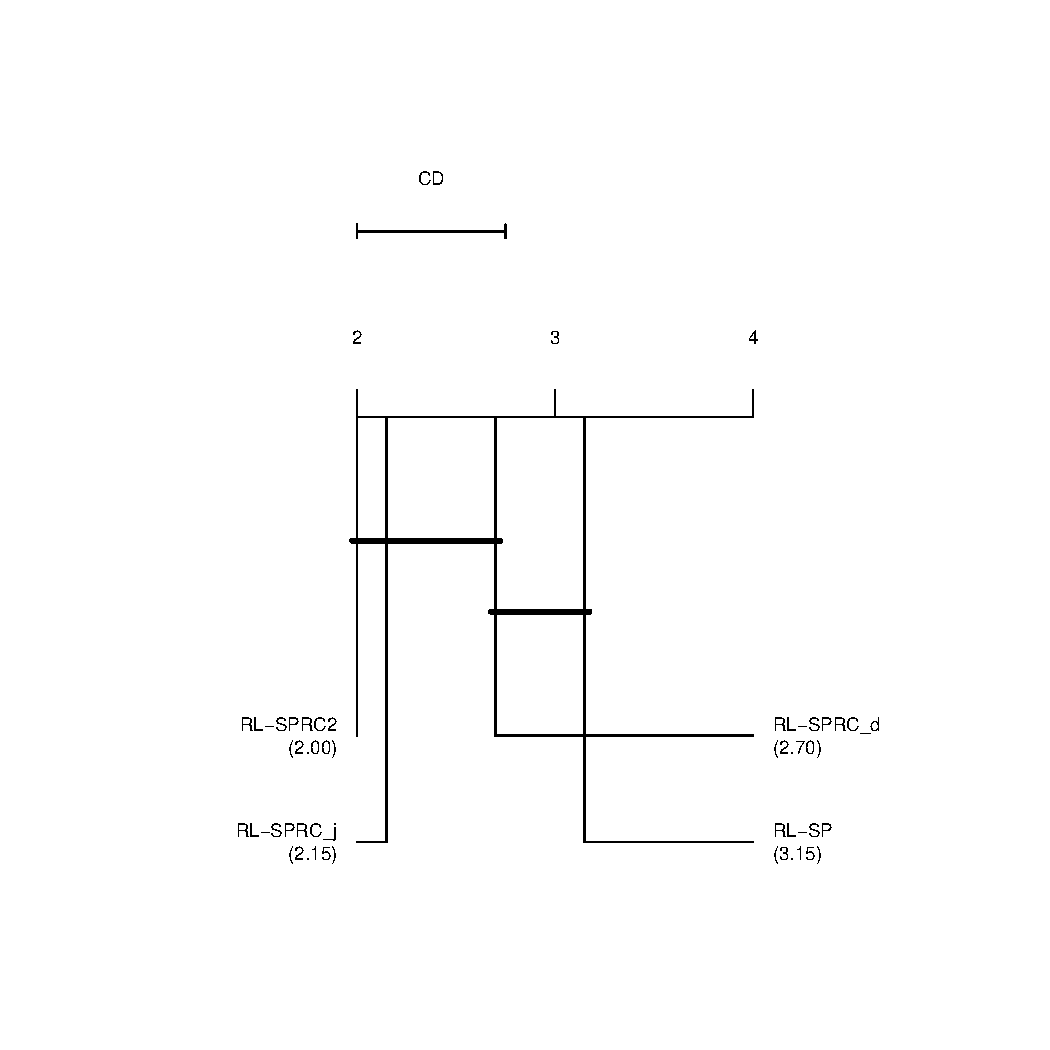
\includegraphics[scale=0.6]{imagens/rls.pdf}
        \vspace*{-2cm}
        \caption{ID = 7.81, VC = 2.68, DC = 0.74}
    \end{subfigure}
    \caption{Testes  de  Iman-Davenport  e   Nemenyi  para  as
diferentes RLs}
    \label{fig:rl-nemenyi}
\end{figure}

Por serem  estatisticamente equivalentes,  no procedimento para  selecionar qual
dentre as  três relaxações é  considerada melhor,  pode-se analisar o  número de
vitórias para cada relaxação, como apresentado na Tabela \ref{tab:contagem-rls}.
A primeira  linha e  coluna referenciam  as relaxações,  cada posição  da tabela
representa o número de vitórias da abordagem referente a linha sobre a abordagem
na coluna.

\begin{table}[!ht]
\centering
\resizebox{\textwidth}{!}{%
\begin{tabular}{llclclclc}
\hline
\multicolumn{1}{c}{Relaxações} & \multicolumn{1}{c}{} & RL-SP & \multicolumn{1}{c}{} & RL-SPRC$_{\lambda}$ & \multicolumn{1}{c}{} & RL-SPRC$_{\xi}$ & \multicolumn{1}{c}{} & RL-SPRC2 \\ \hline
RL-SP &  & - &  & 04 &  & 00 &  & 02 \\
RL-SPRC$_{\lambda}$ &  & 15 &  & - &  & 04 &  & 01 \\
RL-SPRC$_{\xi}$ &  & 22 &  & 14 &  & - &  & 05 \\
RL-SPRC2 &  & 21 &  & 18 &  & 09 &  & - \\ \hline
\end{tabular}%
}
\caption{Contagem de vitórias entre as RLs.}
\label{tab:contagem-rls}
\end{table}

Pela contagem  de vitórias,  observa-se que a  relaxação {\rlq}  teve desempenho
superior  as outras  duas  em uma  quantidade maior  de  instâncias. Enquanto  a
relaxação {\rlu}  obteve os  piores \textit{ranks}  médios e  o menor  número de
vitórias em comparação com demais relaxações. É possível inferir que a qualidade
dos  \gls{ls}s  obtidos com  a  aplicação  da  heurística  de busca  local  está
fortemente  atrelada  com a  qualidade  dos  caminhos  gerados pela  solução  do
\gls{ppl}, pois o  pior \textit{rank} médio está associado com  a relaxação mais
fraca, que por sua vez resulta em um \gls{ppl} cuja solução é menos interessante
do ponto de vista heurístico. A relaxação  contendo maior número de vitórias e o
melhor  \textit{rank} médio,  para  esse  conjunto de  instâncias,  se trata  da
{\rlq}, na  qual o \gls{ppl}  tem a  maior complexidade computacional  dentre as
relaxações propostas. Tais resultados confirmam  que, quanto mais restrições são
mantidas no \gls{ppl}, maior a qualidade do limitantes.

\section{BRKGA}

Na  implementação  dos  decodificadores  para o  \gls{brkga},  foi  utilizada  a
biblioteca Boost  C++ na versão 1.73  para computar a \gls{agm}.  O tempo máximo
para resolução de cada instância foi pré-definido com valor de 1800 segundos (30
minutos). Os valores de parâmetros utilizados no \gls{brkga} foram empiricamente
validados e consistem em:

\begin{itemize}
\item \textbf{População:} são geradas três populações independentes contendo 500
indivíduos cada uma.  O conjunto de elite  é formado por $10\%$  da população. A
cada iteração, $5\%$ dos indivíduos da população são substituídos por mutantes;
\item  \textbf{\textit{Crossover}:}  um novo  indivíduo  é  gerado a  partir  do
cruzamento de  dois indivíduos da  geração atual, um do  conjunto elite e  um do
conjunto não elite. Sendo 70$\%$ de probabilidade do filho herdar o alelo do pai
do conjunto de elite.
\item  \textbf{Gerações:} o  número máximo  de  gerações foi  limitada em  1000,
efetuando a troca dos 2 melhores indivíduos a cada 100 gerações.
\end{itemize}

As  versões do  \gls{brkga} nesta  seção são  diferenciadas principalmente  pela
função de aptidão utilizada (F1, F2 ou F3), mas são consideradas características
adicionais  ao decodificador  como a  adição do  procedimento de  \gls{bl} ou  a
alteração  no  procedimento  de  geração  das  chaves  aleatórias  com  base  na
frequência dos arcos da relaxação lagrangiana (RL).

A  Tabela \ref{tab:brkga-resultados}  contém  os resultados  de  5 variações  do
\gls{brkga}, as duas primeiras  com função de aptidão F1 (``F1'')  e a função de
aptidão F2 (``F2''). A função de aptidão  F3 é utilizada nas 3 outras variações,
respectivamente (``F3''), (``F3-BL'')  e (``F3-RL''). As primeiras  4 colunas da
tabela apresentam,  respectivamente, o nome  da instância, quantidade de  nós do
grafo  (``|V|''), número  de nós  terminais (``|D|'')  e a  quantidade de  arcos
(``|A|''). Para  cada algoritmo  são dispostas duas  colunas: ``LS''  contendo o
número  de terminais  atendidos  na  melhor solução  e  a  coluna ``Tempo''  que
apresenta o tempo de execução em segundos. O valor TLE representa que a execução
atingiu o tempo  limite de execução. Valores em  \textbf{negrito} representam os
melhores \gls{ls}s dentre as versões do \gls{brkga} para cara instância. A linha
``\textbf{Melhor}'' indica o número de instâncias nas quais o algoritmo obteve a
melhor  solução e  que nenhuma  outra variação  atingiu o  mesmo valor.  A linha
``\textbf{Igual}'' contém  o número  de instâncias cujo  limitante foi  igual ao
melhor obtido entre  as demais versões. A linha  ``\textbf{Pior}'' contabiliza o
total  de casos  onde a  solução retornada  pelo decodificador  foi inferior  ao
melhor limitante para a instância.

\newpage

\begin{table}[!ht]
\centering
\resizebox{\textwidth}{!}{%
\begin{tabular}{lrrrrrrrrrrrrrrrrr}
\hline
\multicolumn{1}{c}{\textbf{}} & \multicolumn{1}{c}{\textbf{}} & \multicolumn{1}{c}{\textbf{}} & \multicolumn{1}{c}{\textbf{}} & \multicolumn{2}{c}{\textbf{F1}} & \multicolumn{1}{c}{\textbf{}} & \multicolumn{2}{c}{\textbf{F2}} & \multicolumn{1}{c}{\textbf{}} & \multicolumn{2}{c}{\textbf{F3}} & \multicolumn{1}{c}{\textbf{}} & \multicolumn{2}{c}{\textbf{F3-BL}} & \multicolumn{1}{c}{\textbf{}} & \multicolumn{2}{c}{\textbf{F3-RL}} \\ \cline{5-6} \cline{8-9} \cline{11-12} \cline{14-15} \cline{17-18} 
\multicolumn{1}{c}{\textbf{Instância}} & \multicolumn{1}{c}{\textbf{|V|}} & \multicolumn{1}{c}{\textbf{|D|}} & \multicolumn{1}{c}{\textbf{|E|}} & \multicolumn{1}{c}{\textbf{LS}} & \multicolumn{1}{c}{\textbf{Tempo}} & \multicolumn{1}{c}{\textbf{}} & \multicolumn{1}{c}{\textbf{LS}} & \multicolumn{1}{c}{\textbf{Tempo}} & \multicolumn{1}{c}{\textbf{}} & \multicolumn{1}{c}{\textbf{LS}} & \multicolumn{1}{c}{\textbf{Tempo}} & \multicolumn{1}{c}{\textbf{}} & \multicolumn{1}{c}{\textbf{LS}} & \multicolumn{1}{c}{\textbf{Tempo}} & \multicolumn{1}{c}{\textbf{}} & \multicolumn{1}{c}{\textbf{LS}} & \textbf{Tempo} \\ \hline
washington-50-10-6 & 10 & 6 & 23 & \textbf{1} & 105 &  & \textbf{1} & 108 &  & \textbf{1} & 115 &  & \textbf{1} & 138 &  & \textbf{1} & 191 \\
washington-50-20-11 & 20 & 11 & 92 & \textbf{4} & 328 &  & \textbf{4} & 339 &  & \textbf{4} & 354 &  & \textbf{4} & 399 &  & \textbf{4} & 587 \\
washington-50-30-15 & 30 & 15 & 210 & \textbf{3} & 697 &  & \textbf{3} & 829 &  & \textbf{3} & 829 &  & \textbf{3} & 1.002 &  & \textbf{3} & 1347 \\
washington-50-40-23 & 40 & 23 & 415 & \textbf{6} & 1.453 &  & 7 & TLE &  & \textbf{6} & 1.688 &  & \textbf{6} & 1.651 &  & \textbf{6} & 1683 \\
washington-50-50-28 & 50 & 28 & 624 & \textbf{13} & TLE &  & \textbf{13} & TLE &  & \textbf{13} & TLE &  & \textbf{13} & TLE &  & \textbf{13} & TLE \\
washington-50-60-35 & 60 & 35 & 906 & \textbf{17} & TLE &  & 19 & TLE &  & \textbf{17} & TLE &  & 18 & TLE &  & \textbf{17} & TLE \\
washington-50-70-37 & 70 & 37 & 1258 & \textbf{16} & TLE &  & 18 & TLE &  & \textbf{16} & TLE &  & 17 & TLE &  & \textbf{16} & TLE \\
washington-50-80-39 & 80 & 39 & 1796 & \textbf{29} & TLE &  & \textbf{29} & TLE &  & \textbf{29} & TLE &  & \textbf{29} & TLE &  & \textbf{29} & TLE \\
washington-50-90-51 & 90 & 51 & 2109 & \textbf{36} & TLE &  & \textbf{36} & TLE &  & \textbf{36} & TLE &  & \textbf{36} & TLE &  & \textbf{36} & TLE \\
washington-50-100-45 & 100 & 45 & 2208 & 35 & TLE &  & 35 & TLE &  & \textbf{34} & TLE &  & \textbf{34} & TLE &  & \textbf{34} & TLE \\ \hline
washington-75-10-4 & 10 & 4 & 16 & \textbf{3} & 144 &  & \textbf{3} & 147 &  & \textbf{3} & 100 &  & \textbf{3} & 148 &  & \textbf{3} & 152 \\
washington-75-20-12 & 20 & 12 & 63 & 5 & 413 &  & \textbf{4} & 388 &  & \textbf{4} & 338 &  & \textbf{4} & 513 &  & \textbf{4} & 468 \\
washington-75-30-16 & 30 & 16 & 159 & \textbf{5} & 935 &  & \textbf{5} & 794 &  & \textbf{5} & 742 &  & \textbf{5} & 897 &  & \textbf{5} & 740 \\
washington-75-40-21 & 40 & 21 & 269 & \textbf{5} & 1.127 &  & 8 & 1.172 &  & 6 & 1.228 &  & 6 & 1.351 &  & \textbf{5} & 1183 \\
washington-75-50-30 & 50 & 30 & 438 & \textbf{11} & TLE &  & \textbf{11} & 1.707 &  & \textbf{11} & TLE &  & \textbf{11} & TLE &  & \textbf{11} & TLE \\
washington-75-60-25 & 60 & 25 & 628 & \textbf{11} & TLE &  & 12 & TLE &  & \textbf{11} & TLE &  & \textbf{11} & TLE &  & \textbf{11} & TLE \\
washington-75-70-42 & 70 & 42 & 850 & 23 & TLE &  & 16 & TLE &  & \textbf{13} & TLE &  & \textbf{13} & TLE &  & \textbf{13} & TLE \\
washington-75-80-48 & 80 & 48 & 1252 & 29 & TLE &  & 26 & TLE &  & 13 & TLE &  & \textbf{11} & TLE &  & 13 & TLE \\
washington-75-90-47 & 90 & 47 & 1517 & \textbf{19} & TLE &  & \textbf{19} & TLE &  & \textbf{19} & TLE &  & \textbf{19} & TLE &  & \textbf{19} & TLE \\
washington-75-100-52 & 100 & 52 & 1896 & 28 & TLE &  & 33 & TLE &  & 27 & TLE &  & 28 & TLE &  & \textbf{26} & TLE \\ \hline
washington-100-10-6 & 10 & 6 & 9 & \textbf{2} & 94 &  & \textbf{2} & 95 &  & \textbf{2} & 104 &  & \textbf{2} & 89 &  & \textbf{2} & 105 \\
washington-100-20-10 & 20 & 10 & 49 & \textbf{2} & 272 &  & \textbf{2} & 359 &  & \textbf{2} & 379 &  & \textbf{2} & 285 &  & \textbf{2} & 334 \\
washington-100-30-12 & 30 & 12 & 103 & \textbf{2} & 401 &  & \textbf{2} & 569 &  & \textbf{2} & 573 &  & \textbf{2} & 444 &  & \textbf{2} & 433 \\
washington-100-40-18 & 40 & 21 & 211 & \textbf{4} & 833 &  & \textbf{4} & TLE &  & \textbf{4} & 1.004 &  & \textbf{4} & 1.337 &  & \textbf{4} & 1278 \\
washington-100-50-27 & 50 & 27 & 298 & \textbf{9} & 1.147 &  & \textbf{9} & TLE &  & \textbf{9} & 1.666 &  & \textbf{9} & 1.485 &  & \textbf{9} & TLE \\
washington-100-60-34 & 60 & 34 & 427 & \textbf{10} & 1.620 &  & 11 & TLE &  & \textbf{10} & TLE &  & \textbf{10} & TLE &  & \textbf{10} & TLE \\
washington-100-70-39 & 70 & 39 & 602 & \textbf{24} & TLE &  & \textbf{24} & TLE &  & \textbf{24} & TLE &  & \textbf{24} & TLE &  & \textbf{24} & TLE \\
washington-100-80-32 & 80 & 32 & 882 & 18 & TLE &  & 7 & TLE &  & \textbf{6} & TLE &  & \textbf{6} & TLE &  & \textbf{6} & TLE \\
washington-100-90-43 & 90 & 43 & 1151 & 32 & TLE &  & 20 & TLE &  & \textbf{11} & TLE &  & 13 & TLE &  & \textbf{11} & TLE \\
washington-100-100-43 & 100 & 43 & 1408 & 14 & TLE &  & 13 & TLE &  & \textbf{12} & TLE &  & \textbf{12} & TLE &  & \textbf{12} & TLE \\ \hline
washington-200-125-55 & 125 & 55 & 1224 & 42 & TLE &  & 42 & TLE &  & \textbf{32} & TLE &  & 33 & TLE &  & 33 & TLE \\
washington-200-150-61 & 150 & 61 & 2234 & 41 & TLE &  & 44 & TLE &  & 37 & TLE &  & 37 & TLE &  & \textbf{35} & TLE \\
washington-200-175-74 & 175 & 74 & 3024 & 39 & TLE &  & 42 & TLE &  & 40 & TLE &  & \textbf{38} & TLE &  & 39 & TLE \\
washington-200-200-114 & 200 & 114 & 3645 & 105 & TLE &  & 105 & TLE &  & 88 & TLE &  & 89 & TLE &  & \textbf{75} & TLE \\
washington-200-225-135 & 225 & 135 & 4464 & 79 & TLE &  & 87 & TLE &  & 65 & TLE &  & 73 & TLE &  & \textbf{62} & TLE \\
washington-200-250-109 & 250 & 109 & 6403 & 76 & TLE &  & 83 & TLE &  & 61 & TLE &  & 61 & TLE &  & \textbf{55} & TLE \\
washington-200-275-146 & 275 & 146 & 7195 & 109 & TLE &  & 116 & TLE &  & 104 & TLE &  & 103 & TLE &  & \textbf{101} & TLE \\
washington-200-300-136 & 300 & 136 & 8709 & 116 & TLE &  & 116 & TLE &  & 102 & TLE &  & 100 & TLE &  & \textbf{99} & TLE \\
washington-200-325-170 & 325 & 170 & 9260 & 151 & TLE &  & 154 & TLE &  & 135 & TLE &  & 130 & TLE &  & \textbf{128} & TLE \\
washington-200-350-150 & 350 & 150 & 12218 & 124 & TLE &  & 127 & TLE &  & 98 & TLE &  & 97 & TLE &  & \textbf{96} & TLE \\ \hline
\multicolumn{1}{l}{\textbf{Melhor}} &  &  &  & 0 &  &  & 0 &  &  & 1 &  &  & 2 &  &  & 9 &  \\
\multicolumn{1}{l}{\textbf{Igual}} &  &  &  & 22 &  &  & 17 &  &  & 27 &  &  & 24 &  &  & 28 &  \\
\multicolumn{1}{l}{\textbf{Pior}} &  &  &  & 18 &  &  & 23 &  &  & 12 &  &  & 14 &  &  & 3 &  \\ \hline
\end{tabular}%
}
\caption{Resultados das versões do BRKGA.}
\label{tab:brkga-resultados}
\end{table}

\begin{comment}
Inicialmente para investigar o desempenho das diferentes versões do \gls{brkga} para o conjunto de instâncias, foi utilizado o teste de Iman-Davenport e quando uma diferença estatisticamente significativa (DES) é identificada por esse teste, procedemos com o teste de Nemenyi para detectar grupos de heurísticas equivalentes entre si. Para todos os testes consideramos um nível de confiança de $95\%$, com a hipótese nula de que não existe DES entre todas as heurísticas.

Considerando os valores de \gls{ls} constantes na Tabela \ref{tab:brkga-resultados}, os seguintes resultados foram computados:
\begin{itemize}
    \item O valor de \textit{rank} médio das versões, em ordem crescente, é:
        \begin{itemize}
            \item F3-RL = 2.24
            \item F3 = 2.64
            \item F3-BL = 2.69
            \item F1 = 3.48
            \item F2 = 3.96
        \end{itemize}
    \item Valor de teste de Iman-Davenport = $9.52$;
    \item De acordo com a distribuição, o Valor Crítico = $2.42$;
    \item Segundo o teste de Nemenyi, o valor de Diferença Crítica = $0.97$.
\end{itemize}
\end{comment}

Considerando  os resultados  da  Tabela  \ref{tab:brkga-resultados}, nota-se  um
consumo de tempo  relativamente alto dos decodificadores  independente de função
de aptidão, dado que quase todas as  instâncias contendo 50 ou mais nós, não foi
possível  executar o  \gls{brkga} por  1000 gerações  antes de  atingir o  tempo
limite de 30 minutos. A quantidade de TLEs de cada algoritmo foi bem semelhante,
sendo  {\bfum} a  versão com  menos TLEs,  totalizando 26.  Em contrapartida,  a
versão  {\bfdois} tem  o maior  número  de instâncias  onde o  tempo limite  foi
alcançado, totalizando  29 casos.  O tempo  médio para as  instâncias em  que os
\gls{brkga}s executaram  por 1000 gerações,  se manteve  entre 10 e  12 minutos,
para todas as versões.

A aplicação  do teste  de Iman-Davenport  indicou a existência  de DES  entre as
amostras. Ao aplicar o teste de Nemenyi o resultado agrupou as versões F3, F3-BL
e F3-RL com  os menores valores de  {\em rank} médio, o  que indica equivalência
estatística. Esses dados estão  representados na Figura \ref{fig:brkga-nemenyi},
que também contém o valor computado pelos testes de Iman-Davenport (ID), o Valor
Crítico (VC) e a Diferença Crítica (DC). \newline

%\vspace*{-1.8cm}
\begin{figure}[!ht]
    \centering
    \begin{subfigure}{.5\textwidth}
        \centering
        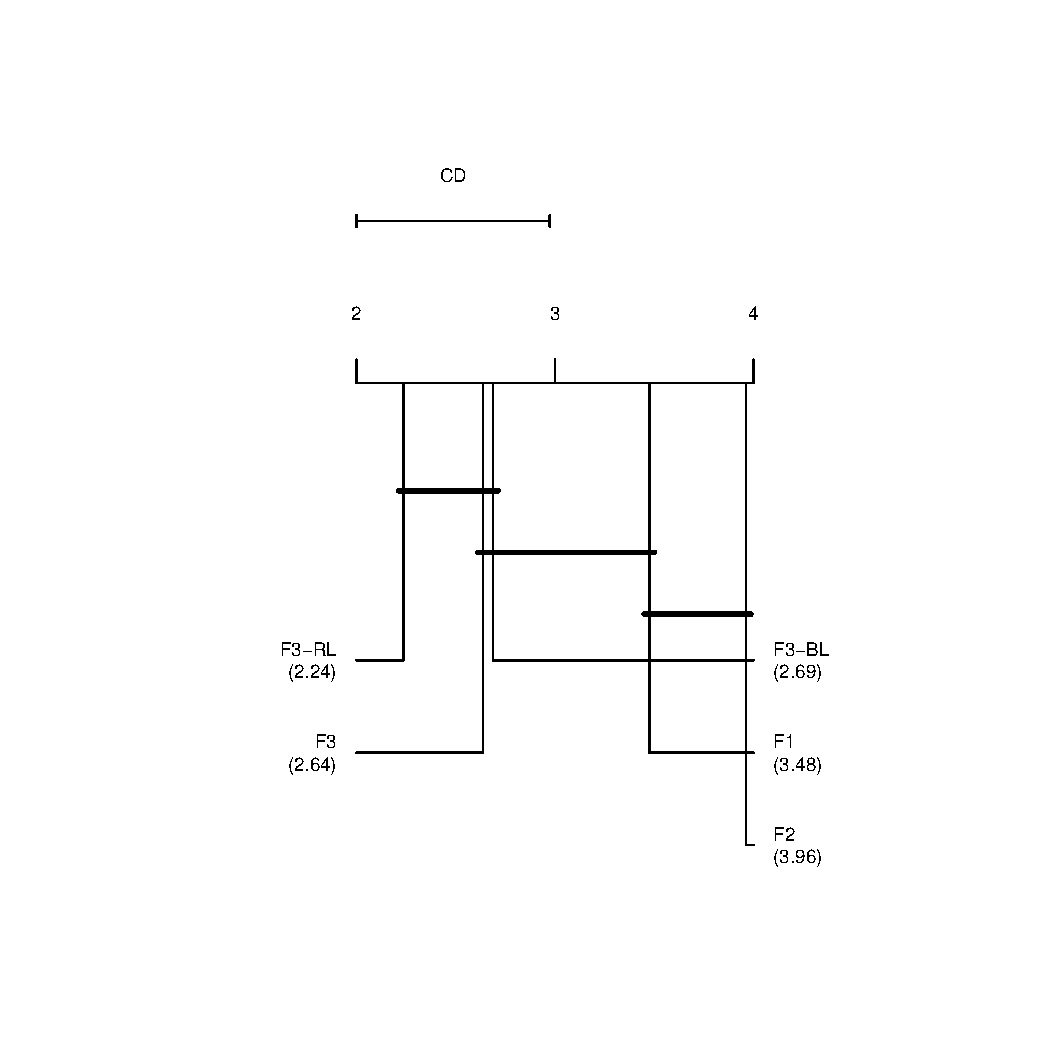
\includegraphics[scale=0.6]{imagens/plot-id.pdf}
        \vspace*{-2cm}
        \caption{ID = 9.52, VC = 2.42, DC = 0.97}
    \end{subfigure}
    \caption{Testes de Imand-Davenport e Nemenyi para os
      decodificadores das versões do BRKGA.}
    \label{fig:brkga-nemenyi}
\end{figure}

Entretanto, ao notar a diferença de {\em rank} médio entre os \gls{brkga}s F3-RL
e F3, optou-se  pela aplicação do teste estatístico de  Wilcoxon para essas duas
variações, motivado pelo fato desse teste estatístico apresentar resultados mais
confiáveis tratando-se apenas de duas amostras. O resultado calculado pelo teste
de Wilcoxon foi $-5.47$, o que significa que existe DES entre as abordagens. Por
fim, além da  diferença estatística, a contagem de vitórias  da versão F3-RL foi
maior, possibilitando  afirmar que  essa versão pode  ser considerada  melhor em
comparação com as demais variações do \gls{brkga}.

Considerando a  capacidade de melhora  das soluções,  é possível observar  que a
versão {\bfdois}, que utiliza a abordagem de soma das penalizações, foi a função
de  aptidão  que  apresentou  os   piores  resultados  dentre  as  5  abordagens
comparadas.  Dentre  as  versões  do   \gls{brkga}  que  obtiveram  os  melhores
resultados, mais especificamente as variações  da função F3, nenhuma dominou por
completo as demais abordagens, ou seja,  não houve um algoritmo cujos resultados
foram melhores em todas as 40 instâncias.

A utilização da busca local não apresentou ganhos significativos, obtendo apenas
6 soluções  melhores que a versão  {\bftres} sem utilizar busca  local, enquanto
gerou  resultados  inferiores   para  outras  7  instâncias.  Já   a  versão  do
decodificador  F3-RL apresentou  \gls{ls}s  com a  maior  qualidade, gerando  as
melhores  soluções para  37 instâncias.  Para as  outras 3  instâncias em  que o
melhor  valor foi  obtido exclusivamente  por  outra versão,  a diferença  entre
resultados foi menor ou igual a 2 terminais. Tais resultados reafirmam a melhora
de qualidade das soluções com base na utilização da informação de frequência dos
arcos selecionados pelo \gls{ppl} na relaxação {\rlq}$^C$.


% k = numero heuristicas
% N = numero de instancias
% Iman-Davenport = 9.52 ($F_f$)
% Valor Crítico = 2.42
% Como o valor encontrado pelo teste ff é maio que o valor crítico, podemos rejeitar a hipótese nula.
% Teste de Nemenyi para computar a diferença crítica e identificar quais grupos de heurísticas que são estatisticamente equivalentes entre si.
% Wilcoxon z < −1.96, podemos rejeitar a hipótese nula.
% Wilcoxon(F3-BL, F3-RL) = -5.47
% Diferença crítica = 0.97 

\newpage

\section{Avaliação Geral dos Limitantes Inferiores} \label{sec:resultados-li}

Esta seção  apresenta a comparação  de todos \gls{li}s obtidos  pelas abordagens
propostas neste  trabalho. Para  tal, serão  considerados os  melhores \gls{li}s
obtidos  pelos modelos  \gls{dmfm-pma}  e \gls{ab-pma},  juntamente dos  valores
retornados por suas respectivas relaxações  lineares e os melhores \gls{li}s das
\gls{rl}s.

A Tabela  \ref{tab:lis-all-comp} contém  os \gls{li}s das  melhores metodologias
utilizadas   nesta   dissertação.   As    primeiras   quatro   colunas   contêm,
respectivamente, o  nome da  instância, o  número de nós  do grafo  (``|V|''), a
quantidade de nós terminais (``|D|'') e  o número de arcos (``|A|''). As colunas
subsequentes  dividem-se entre  as  abordagens, indicando  o  valor de  \gls{li}
obtido  (``LI'') e  o  tempo de  execução em  segundos  (``Tempo''). As  colunas
``\gls{dmfm-pma}'' e  ``\gls{ab-pma}'' apresentam, respectivamente,  os melhores
limitantes     retornados    pelo     resolvedor    \gls{pli}.     As    colunas
``\gls{dmfm-pma}$_{lin}$''  e  ``\gls{ab-pma}$_{lin}$''  contêm  as  respectivas
relaxações  lineares  dos  modelos.  A   última  coluna  apresenta  os  melhores
resultados  da  relaxação {\rlq},  dado  que  esta  \gls{rl} detém  os  melhores
\gls{li}s dentre todas as variações.

\begin{table}[!ht]
\centering
\resizebox{\textwidth}{!}{%
\begin{tabular}{lrrrlrrlrrlrrlrrlrr}
\hline
\multicolumn{1}{c}{} & \multicolumn{1}{c}{} & \multicolumn{1}{c}{} & \multicolumn{1}{c}{} & \multicolumn{1}{c}{} & \multicolumn{2}{c}{\textbf{DMFM-MRP}} & \multicolumn{1}{c}{} & \multicolumn{2}{c}{\textbf{AB-MRP}} & \multicolumn{1}{c}{} & \multicolumn{2}{c}{\textbf{DMFM-MRP$_{lin}$}} & \multicolumn{1}{c}{\textbf{}} & \multicolumn{2}{c}{\textbf{AB-MRP$_{lin}$}} & \multicolumn{1}{c}{\textbf{}} & \multicolumn{2}{c}{\textbf{RL-SPRC2}} \\ \cline{6-7} \cline{9-10} \cline{12-13} \cline{15-16} \cline{18-19} 
\multicolumn{1}{c}{\textbf{Instância}} & \multicolumn{1}{c}{\textbf{|V|}} & \multicolumn{1}{c}{\textbf{|D|}} & \multicolumn{1}{c}{\textbf{|A|}} & \multicolumn{1}{c}{\textbf{}} & \multicolumn{1}{c}{\textbf{LI}} & \multicolumn{1}{c}{\textbf{Tempo}} & \multicolumn{1}{c}{} & \multicolumn{1}{c}{\textbf{LI}} & \multicolumn{1}{c}{\textbf{Tempo}} & \multicolumn{1}{c}{} & \multicolumn{1}{c}{\textbf{LI}} & \multicolumn{1}{c}{\textbf{Tempo}} & \multicolumn{1}{c}{\textbf{}} & \multicolumn{1}{c}{\textbf{LI}} & \multicolumn{1}{c}{\textbf{Tempo}} & \multicolumn{1}{c}{\textbf{}} & \multicolumn{1}{c}{\textbf{LI}} & \multicolumn{1}{c}{\textbf{Tempo}} \\ \hline
washington-50-10-6 & 10 & 6 & 46 &  & \textbf{1} & 0,0 &  & \textbf{1} & 0,0 &  & \textbf{1} & 0,0 &  & 0 & 0,0 &  & \textbf{1} & 0 \\
washington-50-20-11 & 20 & 11 & 184 &  & \textbf{4} & 0,0 &  & \textbf{4} & 0,0 &  & 3 & 0,1 &  & 0 & 0,0 &  & 3 & 34 \\
washington-50-30-15 & 30 & 15 & 420 &  & \textbf{3} & 0,0 &  & \textbf{3} & 0,0 &  & 2 & 0,1 &  & 0 & 0,0 &  & 2 & 75 \\
washington-50-40-23 & 40 & 23 & 830 &  & \textbf{6} & 3,0 &  & \textbf{6} & 4,0 &  & 1 & 0,6 &  & 0 & 0,0 &  & 4 & 786 \\
washington-50-50-28 & 50 & 28 & 1248 &  & \textbf{13} & 3,0 &  & \textbf{13} & 1,0 &  & 7 & 1,0 &  & 0 & 0,0 &  & 6 & 345 \\
washington-50-60-35 & 60 & 35 & 1812 &  & \textbf{15} & 4,0 &  & \textbf{15} & 3,0 &  & 3 & 2,7 &  & 0 & 0,0 &  & 2 & 435 \\
washington-50-70-37 & 70 & 37 & 2516 &  & \textbf{16} & 41,0 &  & \textbf{16} & 26,0 &  & 4 & 4,9 &  & 0 & 0,0 &  & 7 & 823 \\
washington-50-80-39 & 80 & 39 & 3592 &  & \textbf{26} & 25,0 &  & \textbf{26} & 584,0 &  & 23 & 5,1 &  & 0 & 0,0 &  & 23 & 1.336 \\
washington-50-90-51 & 90 & 51 & 4218 &  & \textbf{35} & 285,0 &  & \textbf{35} & 355,0 &  & 18 & 13,4 &  & 0 & 0,0 &  & 19 & 1.790 \\
washington-50-100-45 & 100 & 45 & 4416 &  & \textbf{28} & 71,0 &  & \textbf{28} & 262,0 &  & 12 & 11,8 &  & 0 & 0,0 &  & 16 & TLE \\ \hline
washington-75-10-4 & 10 & 4 & 32 &  & \textbf{3} & 0,0 &  & \textbf{3} & 0,0 &  & 1 & 0,0 &  & 0 & 0,0 &  & 2 & 9 \\
washington-75-20-12 & 20 & 12 & 126 &  & \textbf{4} & 0,0 &  & \textbf{4} & 0,0 &  & 2 & 0,1 &  & 0 & 0,0 &  & 2 & 34 \\
washington-75-30-16 & 30 & 16 & 318 &  & \textbf{5} & 6,0 &  & \textbf{5} & 3,0 &  & 1 & 0,3 &  & 0 & 0,0 &  & 0 & 265 \\
washington-75-40-21 & 40 & 21 & 538 &  & \textbf{5} & 1,0 &  & \textbf{5} & 3,0 &  & \textbf{5} & 0,5 &  & 0 & 0,0 &  & 4 & 209 \\
washington-75-50-30 & 50 & 30 & 876 &  & \textbf{9} & 579,0 &  & \textbf{9} & 2175,0 &  & 3 & 1,0 &  & 0 & 0,0 &  & 3 & 375 \\
washington-75-60-25 & 60 & 25 & 1256 &  & \textbf{11} & 4,0 &  & \textbf{11} & 2,0 &  & 2 & 0,7 &  & 0 & 0,0 &  & 2 & 302 \\
washington-75-70-42 & 70 & 42 & 1700 &  & \textbf{12} & 19,0 &  & \textbf{12} & 136,0 &  & 6 & 5,3 &  & 0 & 0,0 &  & 6 & 856 \\
washington-75-80-48 & 80 & 48 & 2504 &  & \textbf{9} & 42,0 &  & \textbf{9} & 148,0 &  & 2 & 11,1 &  & 0 & 0,0 &  & 2 & 1.292 \\
washington-75-90-47 & 90 & 47 & 3034 &  & \textbf{19} & 89,0 &  & 10 & TLE &  & 3 & 10,7 &  & 0 & 0,0 &  & 3 & 1.448 \\
washington-75-100-52 & 100 & 52 & 3792 &  & \textbf{14} & TLE &  & 13 & TLE &  & 9 & 24,4 &  & 0 & 0,0 &  & 10 & TLE \\ \hline
washington-100-10-6 & 10 & 6 & 18 &  & \textbf{2} & 0,0 &  & \textbf{2} & 0,0 &  & \textbf{2} & 0,0 &  & 0 & 0,0 &  & \textbf{2} & 0 \\
washington-100-20-10 & 20 & 10 & 98 &  & \textbf{2} & 0,0 &  & \textbf{2} & 0,0 &  & 1 & 0,0 &  & 0 & 0,0 &  & 0 & 37 \\
washington-100-30-12 & 30 & 12 & 206 &  & \textbf{2} & 16,0 &  & \textbf{2} & 0,0 &  & 1 & 0,1 &  & 1 & 0,0 &  & \textbf{2} & 90 \\
washington-100-40-18 & 40 & 21 & 422 &  & \textbf{4} & 22,0 & \textbf{} & 4 & 5,0 &  & 1 & 0,5 &  & 0 & 0,0 &  & 1 & 298 \\
washington-100-50-27 & 50 & 27 & 596 &  & 5 & TLE &  & \textbf{9} & 121,0 &  & 1 & 2,7 &  & 0 & 0,0 &  & 1 & 0 \\
washington-100-60-34 & 60 & 34 & 854 &  & \textbf{10} & 3,0 &  & \textbf{10} & 94,0 &  & 7 & 1,2 &  & 0 & 0,0 &  & 7 & 270 \\
washington-100-70-39 & 70 & 39 & 1204 &  & \textbf{17} & 151,0 &  & \textbf{17} & 183,0 &  & 9 & 2,6 &  & 0 & 0,0 &  & 9 & 663 \\
washington-100-80-32 & 80 & 32 & 1764 &  & \textbf{5} & 11,0 &  & \textbf{5} & 23,0 &  & 4 & 3,8 &  & 0 & 0,0 &  & 3 & TLE \\
washington-100-90-43 & 90 & 43 & 2302 &  & \textbf{11} & 107,0 &  & \textbf{11} & 160,0 &  & 3 & 8,6 &  & 0 & 0,0 &  & 2 & 1.216 \\
washington-100-100-43 & 100 & 43 & 2816 &  & \textbf{4} & 146,0 &  & \textbf{4} & 157,0 &  & 2 & 17,3 &  & 0 & 0,0 &  & 1 & 1.513 \\ \hline
washington-200-125-55 & 125 & 55 & 2448 &  & \textbf{29} & 338,0 &  & 27 & TLE &  & 10 & 13,4 &  & 0 & 0,0 &  & 9 & TLE \\
washington-200-150-61 & 150 & 61 & 4468 &  & \textbf{10} & TLE &  & 2 & TLE &  & 7 & 187,4 &  & 0 & 0,1 &  & 7 & TLE \\
washington-200-175-74 & 175 & 74 & 6048 &  & \textbf{20} & TLE &  & 7 & TLE &  & 19 & 2225,4 &  & 0 & 0,1 &  & 18 & TLE \\
washington-200-200-114 & 200 & 114 & 7290 &  & \textbf{32} & TLE &  & 8 & TLE &  & 24 & 730,3 &  & 0 & 0,2 &  & 23 & TLE \\
washington-200-225-135 & 225 & 135 & 8928 &  & 2 & TLE &  & \textbf{8} & TLE &  & 0 & TLE &  & 0 & 0,2 &  & 2 & TLE \\
washington-200-250-109 & 250 & 109 & 12806 &  & 6 & TLE &  & \textbf{11} & TLE &  & 0 & TLE &  & 0 & 0,2 &  & 6 & TLE \\
washington-200-275-146 & 275 & 146 & 14390 &  & \textbf{11} & TLE &  & \textbf{11} & TLE &  & 0 & TLE &  & 0 & 0,2 &  & \textbf{11} & TLE \\
washington-200-300-136 & 300 & 136 & 17418 &  & - & TLE &  & 2 & TLE &  & 0 & TLE &  & 1 & 0,3 &  & \textbf{10} & TLE \\
washington-200-325-170 & 325 & 170 & 18520 &  & - & TLE &  & \textbf{16} & TLE &  & 0 & TLE &  & 0 & 0,4 &  & 13 & TLE \\
washington-200-350-150 & 350 & 150 & 24436 &  & - & TLE &  & \textbf{4} & TLE &  & 0 & TLE &  & 0 & 0,4 &  & \textbf{4} & TLE \\ \hline
\end{tabular}%
}
\caption{Comparação dos melhores LIs entre as metodologias.}
\label{tab:lis-all-comp}
\end{table}

A  aplicação do  teste  de  Iman-Davenport nos  valores  apresentados na  Tabela
\ref{tab:lis-all-comp},  indicou a  presença de  DES entre  as amostras.  Assim,
aplicando  o teste  de  Nemenyi agruparam-se,  com menor  {\em  rank} médio,  os
resultados dos modelos \gls{dmfm-pma} e  \gls{ab-pma}, o que indica equivalência
estatística.     Esses      dados     estão     representados      na     Figura
\ref{fig:all-lis-nemenyi}, que também  contém o valor computado  pelos testes de
Iman-Davenport (ID), o Valor Crítico (VC)  e a Diferença Crítica (DC). Até mesmo
a contagem de  vitórias nos modelos foi igual: cada  um contabilizou 6 vitórias,
enquanto os \gls{li}s foram iguais para as outras 28 instâncias. Ainda assim, os
resultados  dos modelos  não  dominaram  as demais  metodologias  para todas  as
instâncias, ou seja, alguma outra  metodologia apresentou pelo menos um \gls{li}
melhor que ambos os modelos.

\begin{figure}[!ht]
    \centering
    \begin{subfigure}{.5\textwidth}
        \centering
        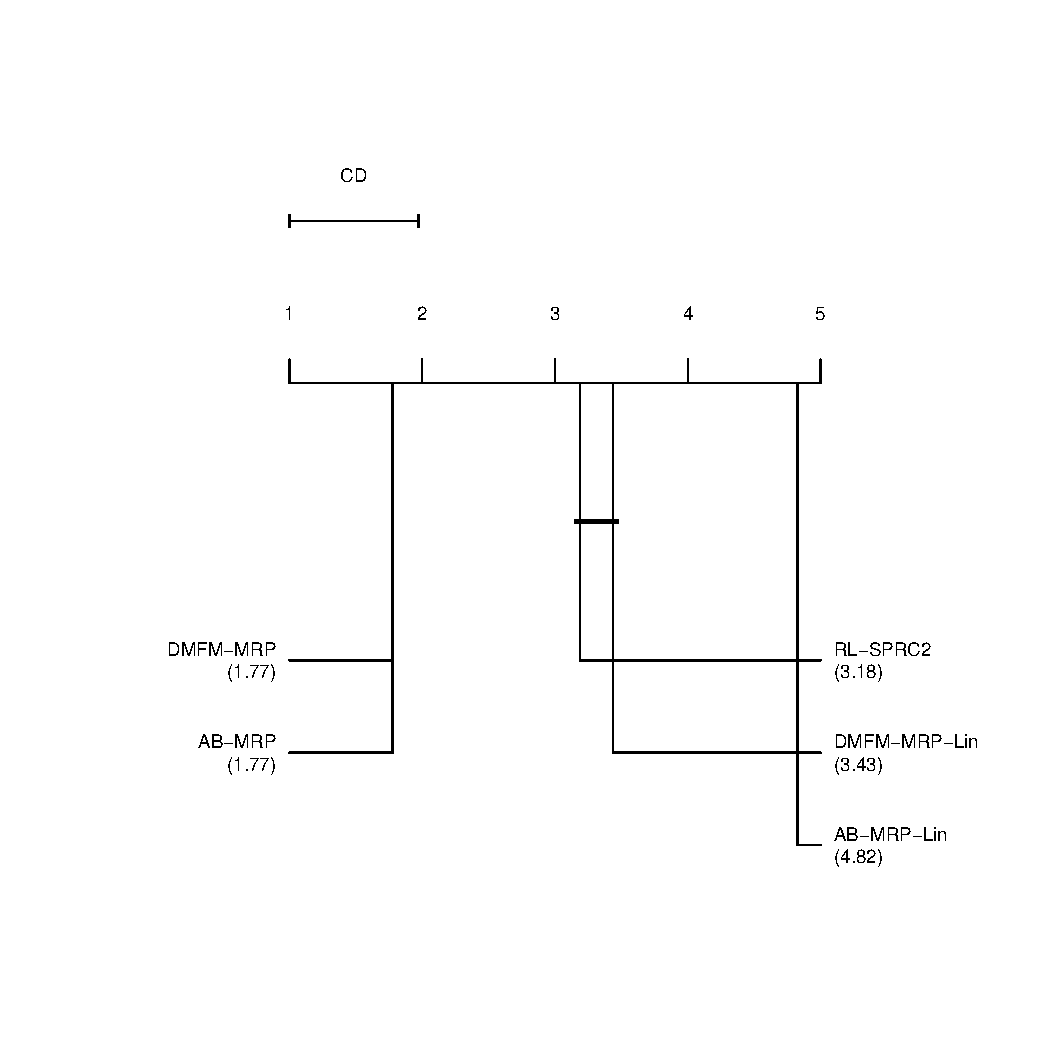
\includegraphics[scale=0.6]{imagens/lis-all.pdf}
        \vspace*{-2cm}
        \caption{ID = 74.32, VC = 2.42, DC = 0.97}
    \end{subfigure}
    \caption{Testes de Iman-Davenport e Nemenyi para os Limitantes Inferiores.}
    \label{fig:all-lis-nemenyi}
\end{figure}

Analisando as  relaxações lineares e a  \gls{rl}, tornou-se evidente a  falta de
qualidade dos limitantes obtidos pela relaxação linear do modelo \gls{ab-pma}. O
valor da relaxação do \gls{ab-pma} para 38 instâncias foi igual a 0 e nas outras
duas instâncias, o resultado foi 1.  A relaxação linear do modelo \gls{dmfm-pma}
apresentou  melhor qualidade,  sendo  estatisticamente  equivalente à  relaxação
{\rlq}.  Entretanto, ao  considerar  a  contagem de  vitórias  entre essas  duas
abordagens, pode-se assumir que {\rlq}  foi melhor. Dado que {\rlq} contabilizou
vitória em 13  instâncias e {\gls{dmfm-pma}$_{lin}$} em apenas 11.  Com base nos
resultados e análises apresentados, notou-se  o excelente desempenho dos modelos
matemáticos, de modo que eles detêm os melhores \gls{li}s para 39 instâncias.

\section{Avaliação Geral dos Limitantes Superiores} \label{sec:resultados-li}

Esta seção apresenta a comparação de todos os \gls{ls}s obtidos pelas diferentes
abordagens propostas  nesse trabalho. Para  tal, serão considerados  os melhores
\gls{ls}s  dos   modelos  \gls{dmfm-pma},  \gls{ab-pma},  a   melhor  versão  do
\gls{brkga} e da \gls{rl}.

A Tabela \ref{tab:ls-all-comp} apresenta  os \gls{ls}s das melhores metodologias
utilizadas   nesta   dissertação.   As    primeiras   quatro   colunas   contém,
respectivamente, o  nome da  instância, o  número de nós  do grafo  (``|V|''), a
quantidade de nós terminais (``|D|'') e  o número de arcos (``|A|''). As colunas
subsequentes  dividem-se entre  as  abordagens, indicando  o  valor de  \gls{ls}
(``LS'')  obtido e  o  tempo de  execução em  segundos  (``Tempo''). As  colunas
``\gls{dmfm-pma}''  e  ``\gls{ab-pma}''  contém,  respectivamente,  os  melhores
\gls{ls}  retornados  pelo  resolvedor  \gls{pli} para  cada  modelo.  A  coluna
``{\rlq}''  contém os  resultados associados  com a  \gls{rl} que  apresentou os
melhores  resultados. Por  fim,  a coluna  ``BRKGA-F3-RL''  dispõe os  \gls{ls}s
retornados pela melhor versão do \gls{brkga}.

\begin{table}[!ht] \centering \resizebox{\textwidth}{!}{%
\begin{tabular}{lrrrlrrlrrlrrlrr}
\hline
\multicolumn{1}{c}{\textbf{}} & \multicolumn{1}{c}{\textbf{}} & \multicolumn{1}{c}{\textbf{}} & \multicolumn{1}{c}{\textbf{}} & \multicolumn{1}{c}{\textbf{}} & \multicolumn{2}{c}{\textbf{DMFM-MRP}} & \multicolumn{1}{c}{\textbf{}} & \multicolumn{2}{c}{\textbf{AB-MRP}} & \multicolumn{1}{c}{\textbf{}} & \multicolumn{2}{c}{\textbf{RL-CRSP2}} & \multicolumn{1}{c}{\textbf{}} & \multicolumn{2}{c}{\textbf{BRKGA-F3-RL}} \\ \cline{6-7} \cline{9-10} \cline{12-13} \cline{15-16} 
\multicolumn{1}{c}{\textbf{Instância}} & \multicolumn{1}{c}{\textbf{|V|}} & \multicolumn{1}{c}{\textbf{|D|}} & \multicolumn{1}{c}{\textbf{|A|}} & \multicolumn{1}{c}{\textbf{}} & \multicolumn{1}{c}{\textbf{LS}} & \multicolumn{1}{c}{\textbf{Tempo}} & \multicolumn{1}{c}{\textbf{}} & \multicolumn{1}{c}{\textbf{LS}} & \multicolumn{1}{c}{\textbf{Tempo}} & \multicolumn{1}{c}{\textbf{}} & \multicolumn{1}{c}{\textbf{LS}} & \multicolumn{1}{c}{\textbf{Tempo}} & \multicolumn{1}{c}{\textbf{}} & \multicolumn{1}{c}{\textbf{LS}} & \multicolumn{1}{c}{\textbf{Tempo}} \\ \hline
washington-50-10-6 & 11 & 6 & 46 &  & \textbf{1} & 0 &  & \textbf{1} & 0 &  & \textbf{1} & 9 &  & \textbf{1} & 191 \\
washington-50-20-11 & 21 & 11 & 184 &  & \textbf{4} & 0 &  & \textbf{4} & 0 &  & \textbf{4} & 32 &  & \textbf{4} & 587 \\
washington-50-30-15 & 31 & 15 & 420 &  & \textbf{3} & 0 &  & \textbf{3} & 0 &  & \textbf{3} & 70 &  & \textbf{3} & 1.347 \\
washington-50-40-23 & 41 & 23 & 830 &  & \textbf{6} & 3 &  & \textbf{6} & 4 &  & \textbf{6} & 158 &  & \textbf{6} & 1.683 \\
washington-50-50-28 & 51 & 28 & 1248 &  & \textbf{13} & 3 &  & \textbf{13} & 1 &  & \textbf{13} & 240 &  & \textbf{13} & TLE \\
washington-50-60-35 & 61 & 35 & 1812 &  & \textbf{15} & 4 &  & \textbf{15} & 3 &  & \textbf{15} & 429 &  & 17 & TLE \\
washington-50-70-37 & 71 & 37 & 2516 &  & \textbf{16} & 41 &  & \textbf{16} & 26 &  & \textbf{16} & 790 &  & \textbf{16} & TLE \\
washington-50-80-39 & 81 & 39 & 3592 &  & \textbf{26} & 25 &  & \textbf{26} & 584 &  & 27 & 860 &  & 29 & TLE \\
washington-50-90-51 & 91 & 51 & 4218 &  & \textbf{35} & 285 &  & \textbf{35} & 355 &  & \textbf{35} & 1.708 &  & 36 & TLE \\
washington-50-100-45 & 101 & 45 & 4416 &  & \textbf{28} & 71 &  & \textbf{28} & 262 &  & 29 & 1.305 &  & 34 & TLE \\ \hline
washington-75-10-4 & 11 & 4 & 32 &  & \textbf{3} & 0 &  & \textbf{3} & 0 &  & \textbf{3} & 9 &  & \textbf{3} & 152 \\
washington-75-20-12 & 21 & 12 & 126 &  & \textbf{4} & 0 &  & \textbf{4} & 0 &  & \textbf{4} & 29 &  & \textbf{4} & 468 \\
washington-75-30-16 & 31 & 16 & 318 &  & \textbf{5} & 6 &  & \textbf{5} & 3 &  & \textbf{5} & 67 &  & \textbf{5} & 740 \\
washington-75-40-21 & 41 & 21 & 538 &  & \textbf{5} & 1 &  & \textbf{5} & 3 &  & 6 & 112 &  & \textbf{5} & 1.183 \\
washington-75-50-30 & 51 & 30 & 876 &  & \textbf{9} & 579 &  & \textbf{9} & 2.175 &  & \textbf{9} & 249 &  & 11 & TLE \\
washington-75-60-25 & 61 & 25 & 1256 &  & \textbf{11} & 4 &  & \textbf{11} & 2 &  & \textbf{11} & 276 &  & \textbf{11} & TLE \\
washington-75-70-42 & 71 & 42 & 1700 &  & \textbf{12} & 19 &  & \textbf{12} & 136 &  & 13 & 677 &  & 13 & TLE \\
washington-75-80-48 & 81 & 48 & 2504 &  & \textbf{9} & 42 &  & \textbf{9} & 148 &  & 10 & 1.186 &  & 13 & TLE \\
washington-75-90-47 & 91 & 47 & 3034 &  & \textbf{19} & 89 &  & \textbf{19} & TLE &  & \textbf{19} & 1.299 &  & \textbf{19} & TLE \\
washington-75-100-52 & 101 & 52 & 3792 &  & 52 & TLE &  & \textbf{20} & TLE &  & 27 & TLE &  & 26 & TLE \\ \hline
washington-100-10-6 & 11 & 6 & 18 &  & \textbf{2} & 0 &  & \textbf{2} & 0 &  & 1 & 8 &  & \textbf{2} & 105 \\
washington-100-20-10 & 21 & 10 & 98 &  & \textbf{2} & 0 &  & \textbf{2} & 0 &  & \textbf{2} & 26 &  & \textbf{2} & 334 \\
washington-100-30-12 & 31 & 12 & 206 &  & \textbf{2} & 16 &  & \textbf{2} & 0 &  & \textbf{2} & 48 &  & \textbf{2} & 433 \\
washington-100-40-18 & 41 & 21 & 422 &  & \textbf{4} & 22 &  & \textbf{4} & 5 &  & 5 & 113 &  & \textbf{4} & 1.278 \\
washington-100-50-27 & 51 & 27 & 596 &  & \textbf{9} & TLE &  & \textbf{9} & 121 &  & 10 & 230 &  & \textbf{9} & TLE \\
washington-100-60-34 & 61 & 34 & 854 &  & \textbf{10} & 3 &  & \textbf{10} & 94 &  & \textbf{10} & 252 &  & \textbf{10} & TLE \\
washington-100-70-39 & 71 & 39 & 1204 &  & \textbf{17} & 151 &  & \textbf{17} & 183 &  & \textbf{17} & 455 &  & 24 & TLE \\
washington-100-80-32 & 81 & 32 & 1764 &  & \textbf{5} & 11 &  & \textbf{5} & 23 &  & 7 & 555 &  & 6 & TLE \\
washington-100-90-43 & 91 & 43 & 2302 &  & \textbf{11} & 107 &  & \textbf{11} & 160 &  & 12 & 904 &  & \textbf{11} & TLE \\
washington-100-100-43 & 101 & 43 & 2816 &  & \textbf{4} & 146 &  & \textbf{4} & 157 &  & 6 & 1.207 &  & 12 & TLE \\ \hline
washington-200-125-55 & 126 & 55 & 2448 &  & \textbf{29} & 338 &  & \textbf{29} & TLE &  & 32 & 1.158 &  & 33 & TLE \\
washington-200-150-61 & 151 & 61 & 4468 &  & 61 & TLE &  & 36 & TLE &  & \textbf{32} & TLE &  & 35 & TLE \\
washington-200-175-74 & 176 & 74 & 6048 &  & 74 & TLE &  & \textbf{37} & TLE &  & 40 & TLE &  & 39 & TLE \\
washington-200-200-114 & 201 & 114 & 7290 &  & 114 & TLE &  & 105 & TLE &  & \textbf{70} & TLE &  & 75 & TLE \\
washington-200-225-135 & 226 & 135 & 8928 &  & - & TLE &  & \textbf{15} & TLE &  & 49 & TLE &  & 62 & TLE \\
washington-200-250-109 & 251 & 109 & 12806 &  & - & TLE &  & \textbf{19} & TLE &  & 45 & TLE &  & 55 & TLE \\
washington-200-275-146 & 276 & 146 & 14390 &  & - & TLE &  & \textbf{71} & TLE &  & 90 & TLE &  & 101 & TLE \\
washington-200-300-136 & 301 & 136 & 17418 &  & - & TLE &  & \textbf{61} & TLE &  & 83 & TLE &  & 99 & TLE \\
washington-200-325-170 & 326 & 170 & 18520 &  & - & TLE &  & \textbf{77} & TLE &  & 114 & TLE &  & 128 & TLE \\
washington-200-350-150 & 351 & 150 & 24436 &  & - & TLE &  & \textbf{45} & TLE &  & 71 & TLE &  & 96 & TLE \\ \hline
\end{tabular}%
}
\caption{Comparação dos melhores LSs entre as metodologias.}
\label{tab:ls-all-comp}
\end{table}

A aplicação do teste de Iman-Davenport  nos valores de limitante apresentados na
tabela \ref{tab:ls-all-comp}, indicaram DES entre as amostras. Assim, agrupou-se
com  base   no  teste   de  Nemenyi,  as   abordagens  \gls{ab-pma},   {\rlq}  e
\gls{dmfm-pma}  com   os  menores   {\em  ranks}   médios.  Esses   dados  estão
representados  na Figura  \ref{fig:all-ls-nemenyi},  que também  contém o  valor
computado  pelos  testes de  Iman-Davenport  (ID),  o  Valor  Crítico (VC)  e  a
Diferença  Crítica (DC).  Entretanto, diante  da diferença  de {\em  rank} médio
entre o  modelo \gls{ab-pma} e  a relaxação  {\rlq}, optou-se pela  aplicação do
teste estatístico  de Wilcoxon, que  indicou a existência  de DES entre  as duas
amostras. Com  isso, pode-se  considerar que o  modelo \gls{ab-pma}  consiste na
melhor abordagem para obtenção de \gls{ls}s. Entretanto, não houve domínio total
sobre todas  as demais  abordagens, ou  seja, não  houve nenhum  algoritmo cujos
resultados foram os melhores para todas as 40 instâncias.

\begin{figure}[!ht] \centering
    \begin{subfigure}{.5\textwidth}
        \centering
        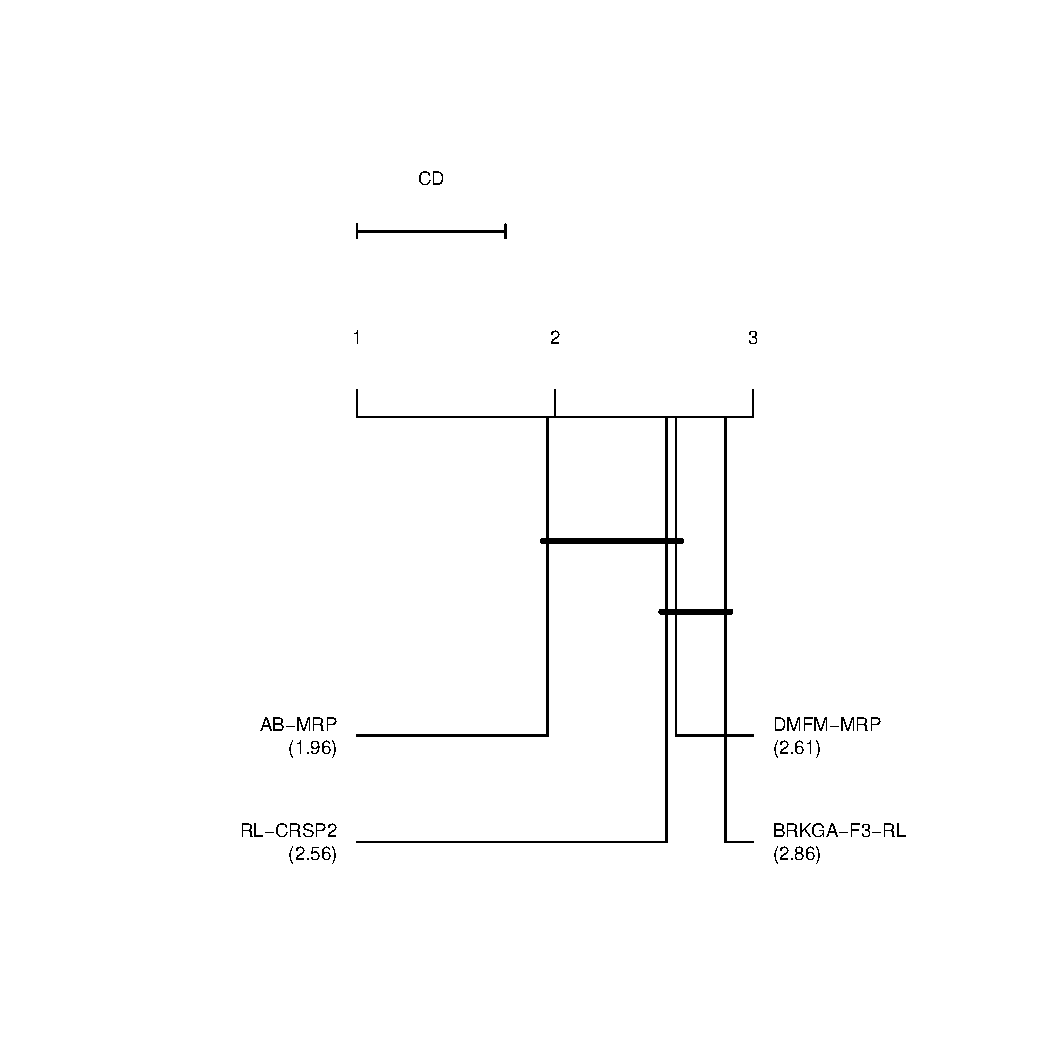
\includegraphics[scale=0.6]{imagens/ls_all.pdf}
        \vspace*{-2cm}
        \caption{ID = 3.73, VC = 2.68, DC = 0.74}
    \end{subfigure}
    \caption{Testes de Iman-Davenport e Nemenyi para os Limitantes Superiores.}
    \label{fig:all-ls-nemenyi}
\end{figure}

O  modelo  \gls{ab-pma}  obteve  o   melhor  desempenho  dentre  as  abordagens,
garantindo  \gls{ls}s  melhores  ou  iguais   às  demais  metodologias  para  37
instâncias do conjunto. Mais especificamente, em 8 instâncias o valor obtido foi
melhor dentre  todos os algoritmos.  Considerando o modelo  \gls{dmfm-pma}, cujo
valor de {\em  rank} médio está bem  próximo ao {\em rank}  da relaxação {\rlq},
observa-se que  a contagem de  vitórias entre eles  foi idêntica, 11  casos para
cada um. Por fim, temos os resultados da versão do \gls{brkga} F3-RL, que obteve
limitantes iguais aos melhores obtidos pelas demais abordagens em 18 instâncias,
mas que, ainda assim, manteve-se no pior \textit{rank} médio.

